
We now calculate the $\WW$ production cross section in each lepton channel
separately, according to equation \ref{eq:mainformula}.
In all cases, the integrated luminosity of the data sample is taken to
be {${\cal{L}} = 4630 \pm 208 \ipb$}, 
and the branching ratio $BR(WW \to \ell \nu) =$ 0.1080 $\pm$ 0.0009~\cite{pdg}.
The efficiency to select ${WW\to 2\ell 2\nu}$
candidates, $\varepsilon$, is computed as the weighted mean of
the $qq\to\WW$ and $gg\to\WW$ efficiencies in simulation,
assuming a 3\% contribution from the $gg$ process.
The results are tabulated in the following sub-sections, and summarised
in Figure \ref{fig:xsec_per_channel}.

\begin{figure}[!hbtp]
\centering
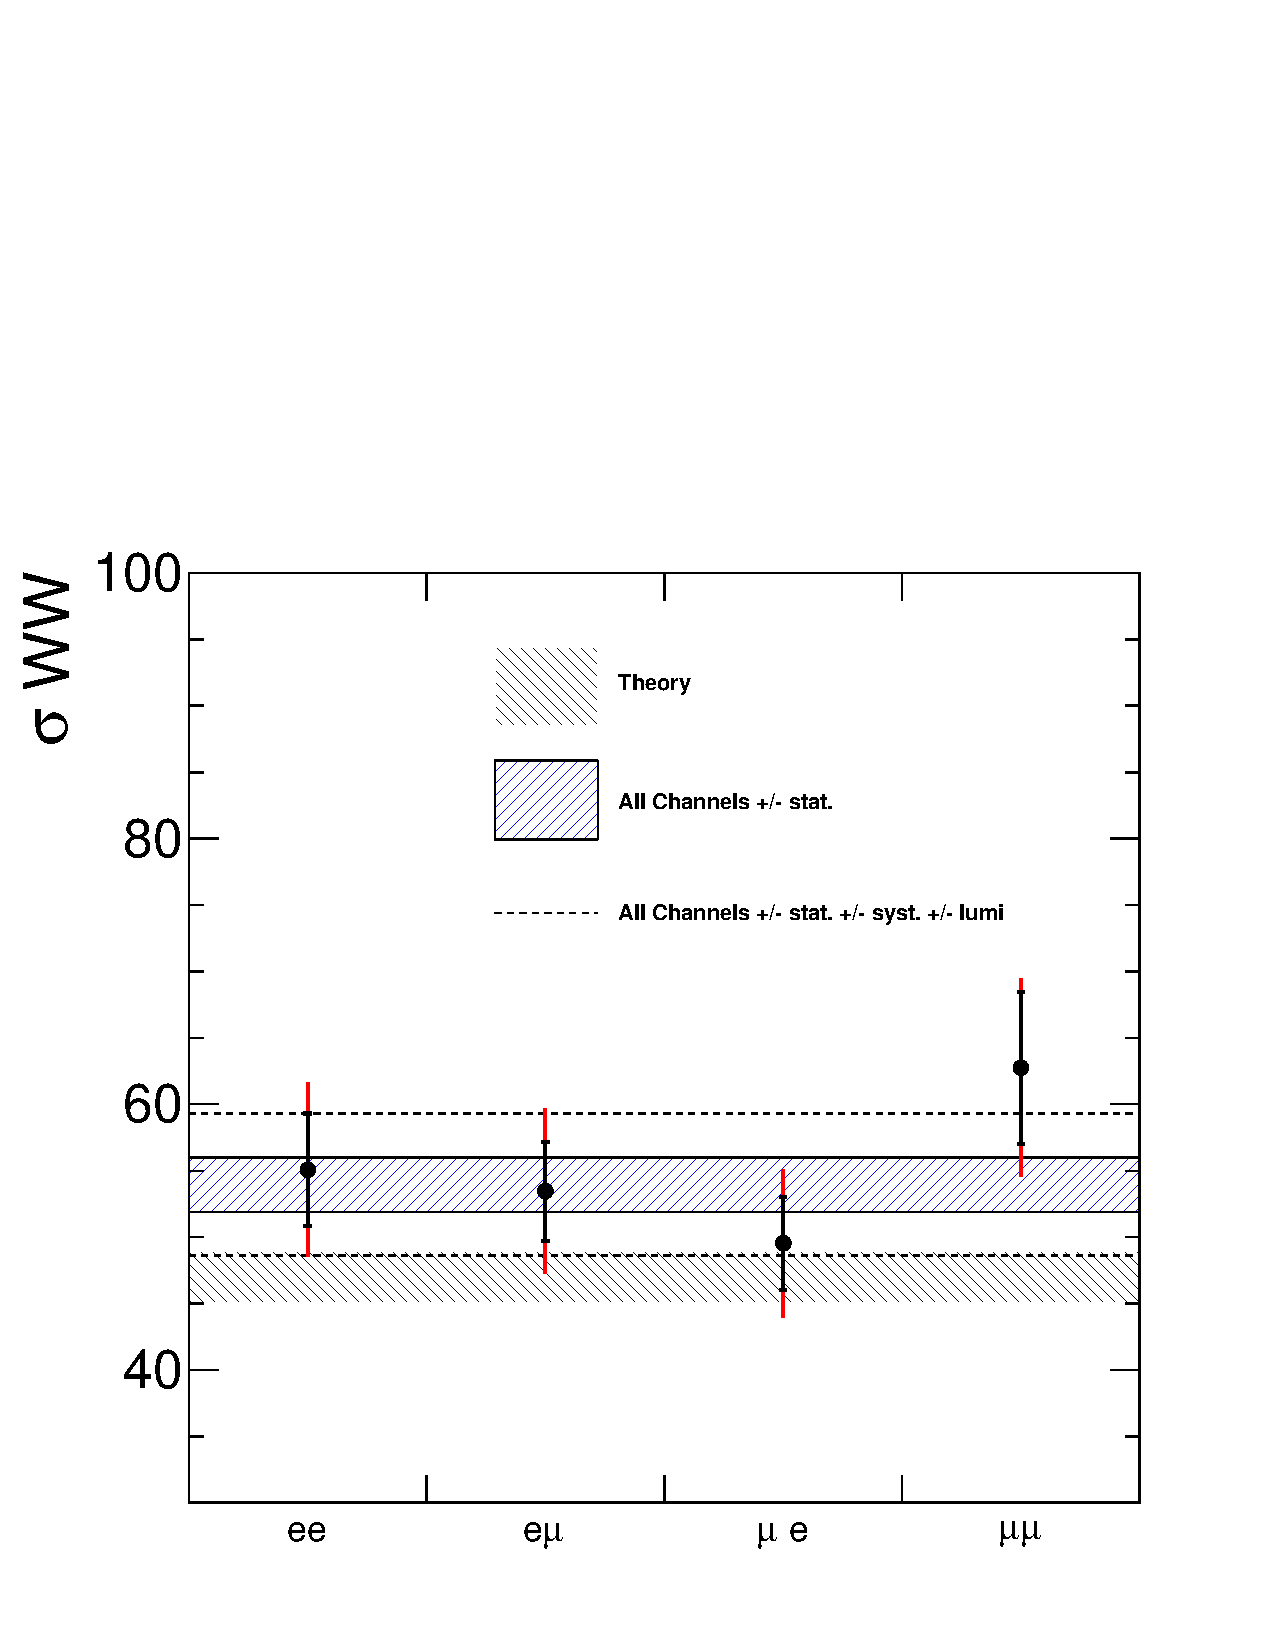
\includegraphics[width=.7\textwidth]{figures/compare_channels.pdf}
\caption{
The cross section measured in each lepton channel compared to the nominal result
combining all channels and the theoretical prediction.
}
\label{fig:xsec_per_channel}
\end{figure}

%
%
%
\clearpage
\subsection{$\mu \mu$ Channel}

The number of events observed and the background predictions and their uncertainties are
given in Table \ref{tab:data_yields_mm}.
The distributions of the $p_{T}$ of the leading and trailing leptons, and the dilepton $p_{T}$
and invariant mass are shown in Figure \ref{fig:mmplots}.
The signal efficiency,  $\varepsilon = 0.00788 \pm 0.00055~\mathrm{(syst.)}$.
The statistical uncertainty on the signal efficiency is negligible.
We obtain the following $WW$ cross-section measurement:

\begin{equation*}
\sigma_{WW}  = 55.07 \pm 4.23~\mathrm{(stat.)} \pm 4.30~\mathrm{(syst.)} \pm 2.48~\mathrm{(lumi.)~pb}.
\end{equation*}

\begin{table}[ht!]
  \begin{center}
  \begin{tabular} {|c|c|}
\hline
Sample                & Yield $\pm$ stat $\pm$ syst \\ \hline \hline
$qqWW$                & 170.1 $\pm$  2.0 $\pm$ 10.7  \\ \hline
$ggWW$                & 10.0 $\pm$  0.3 $\pm$  3.0  \\ \hline
$t\bar{t} + tW$      & 28.3 $\pm$  1.1 $\pm$  5.3  \\ \hline
$W+jets$              &  6.2 $\pm$  2.0 $\pm$  2.2  \\ \hline
$WZ$/$ZZ$             & 10.5 $\pm$  0.3 $\pm$  0.7  \\ \hline
$Z/\gamma*$          &  5.7 $\pm$  2.2 $\pm$  2.5  \\ \hline
$W\gamma*/W+\gamma$ &  1.3 $\pm$  0.8 $\pm$  0.3  \\ \hline \hline
Total Bkgd.           & 52.0 $\pm$  3.3 $\pm$  6.3  \\ \hline \hline
Total Bkgd.+Signal    & 232.1 $\pm$  3.8 $\pm$ 12.8  \\ \hline \hline
Data                  & 263 \\ \hline
\end{tabular}
  \caption{Expected number of signal and background events from the data-driven methods for
  an integrated luminosity of \intlumi after applying the selection requirements in the $mm$ channel.}
   \label{tab:data_yields_mm}
  \end{center}
\end{table}

%%%%%%%%
\begin{figure}[!hbtp]
\begin{center}
\subfigure[Leading lepton $p_{T}$]{\label{subfig:fig_mmplots_pt1}
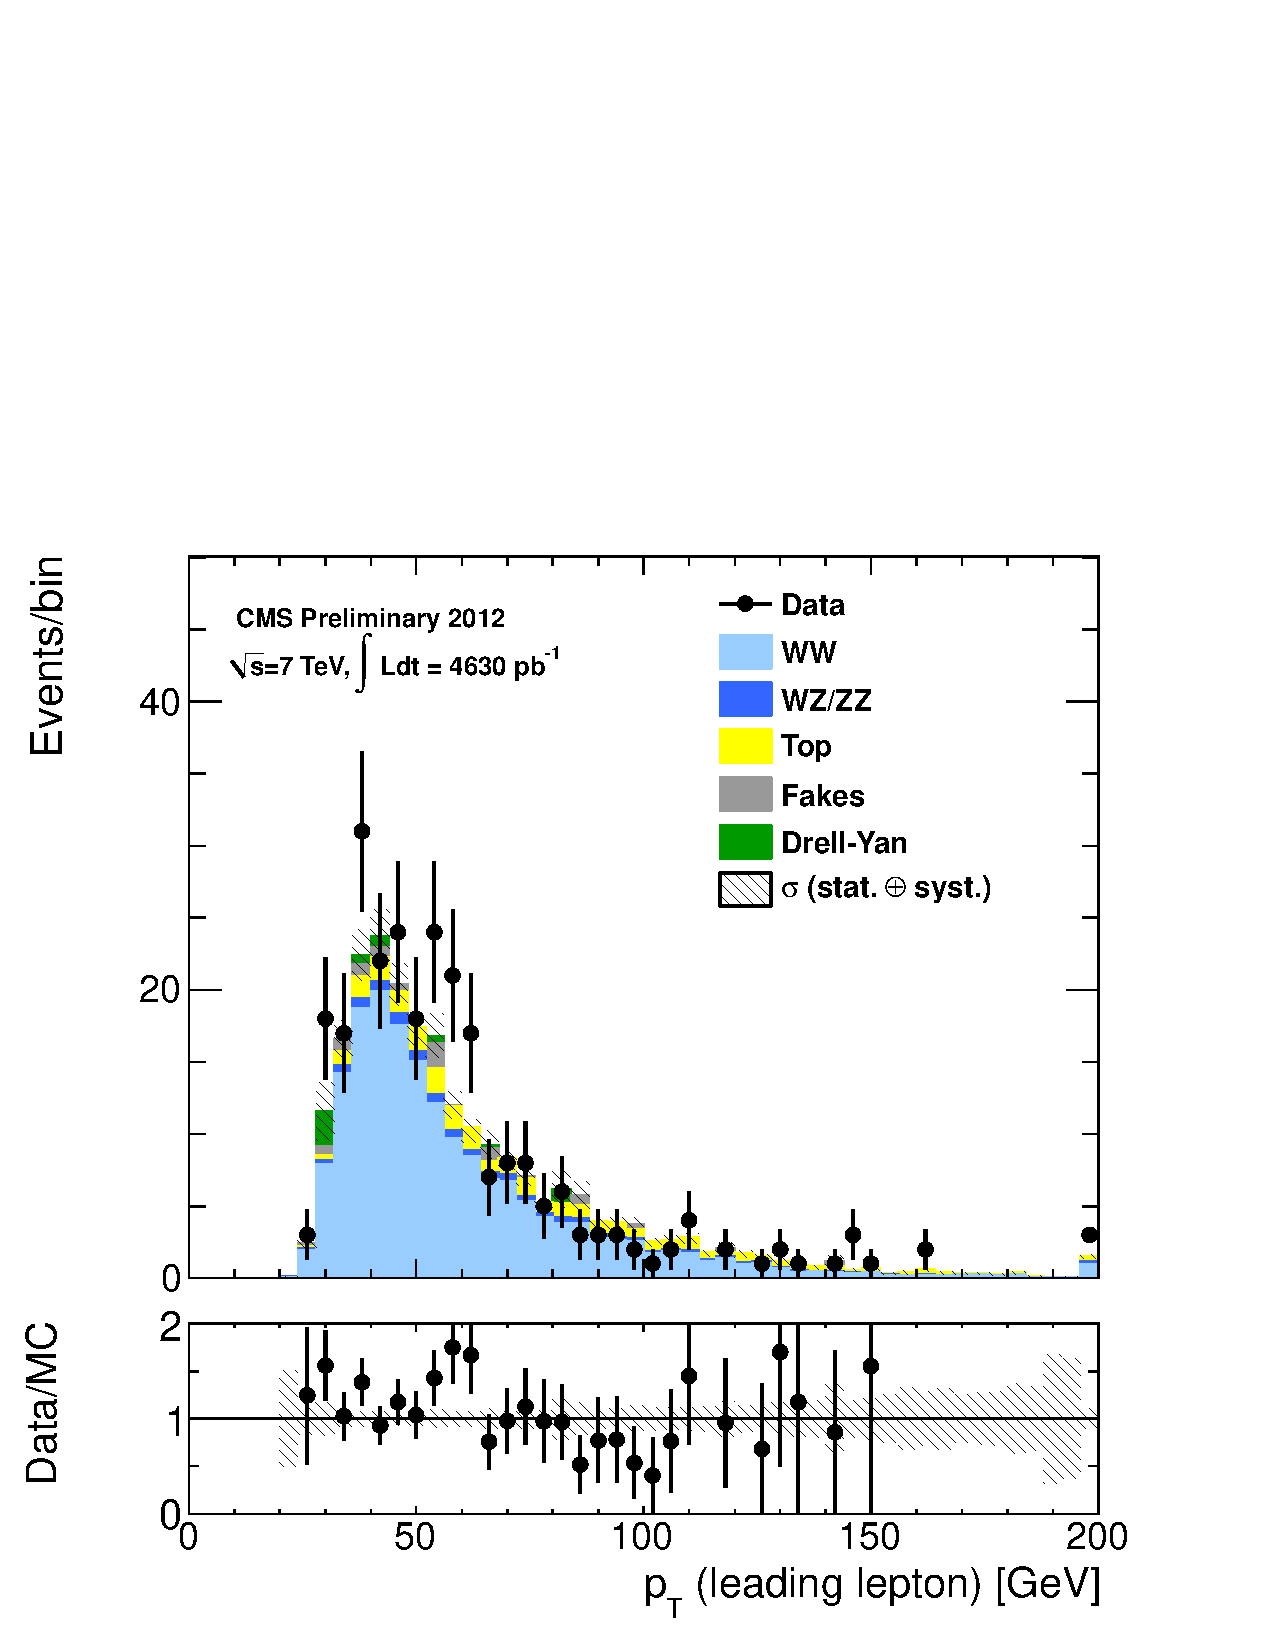
\includegraphics[width=.45\textwidth]{figures/pas_pt1_mm.pdf}}
\subfigure[Trailing lepton $p_{T}$]{\label{subfig:fig_mmplots_pt2}
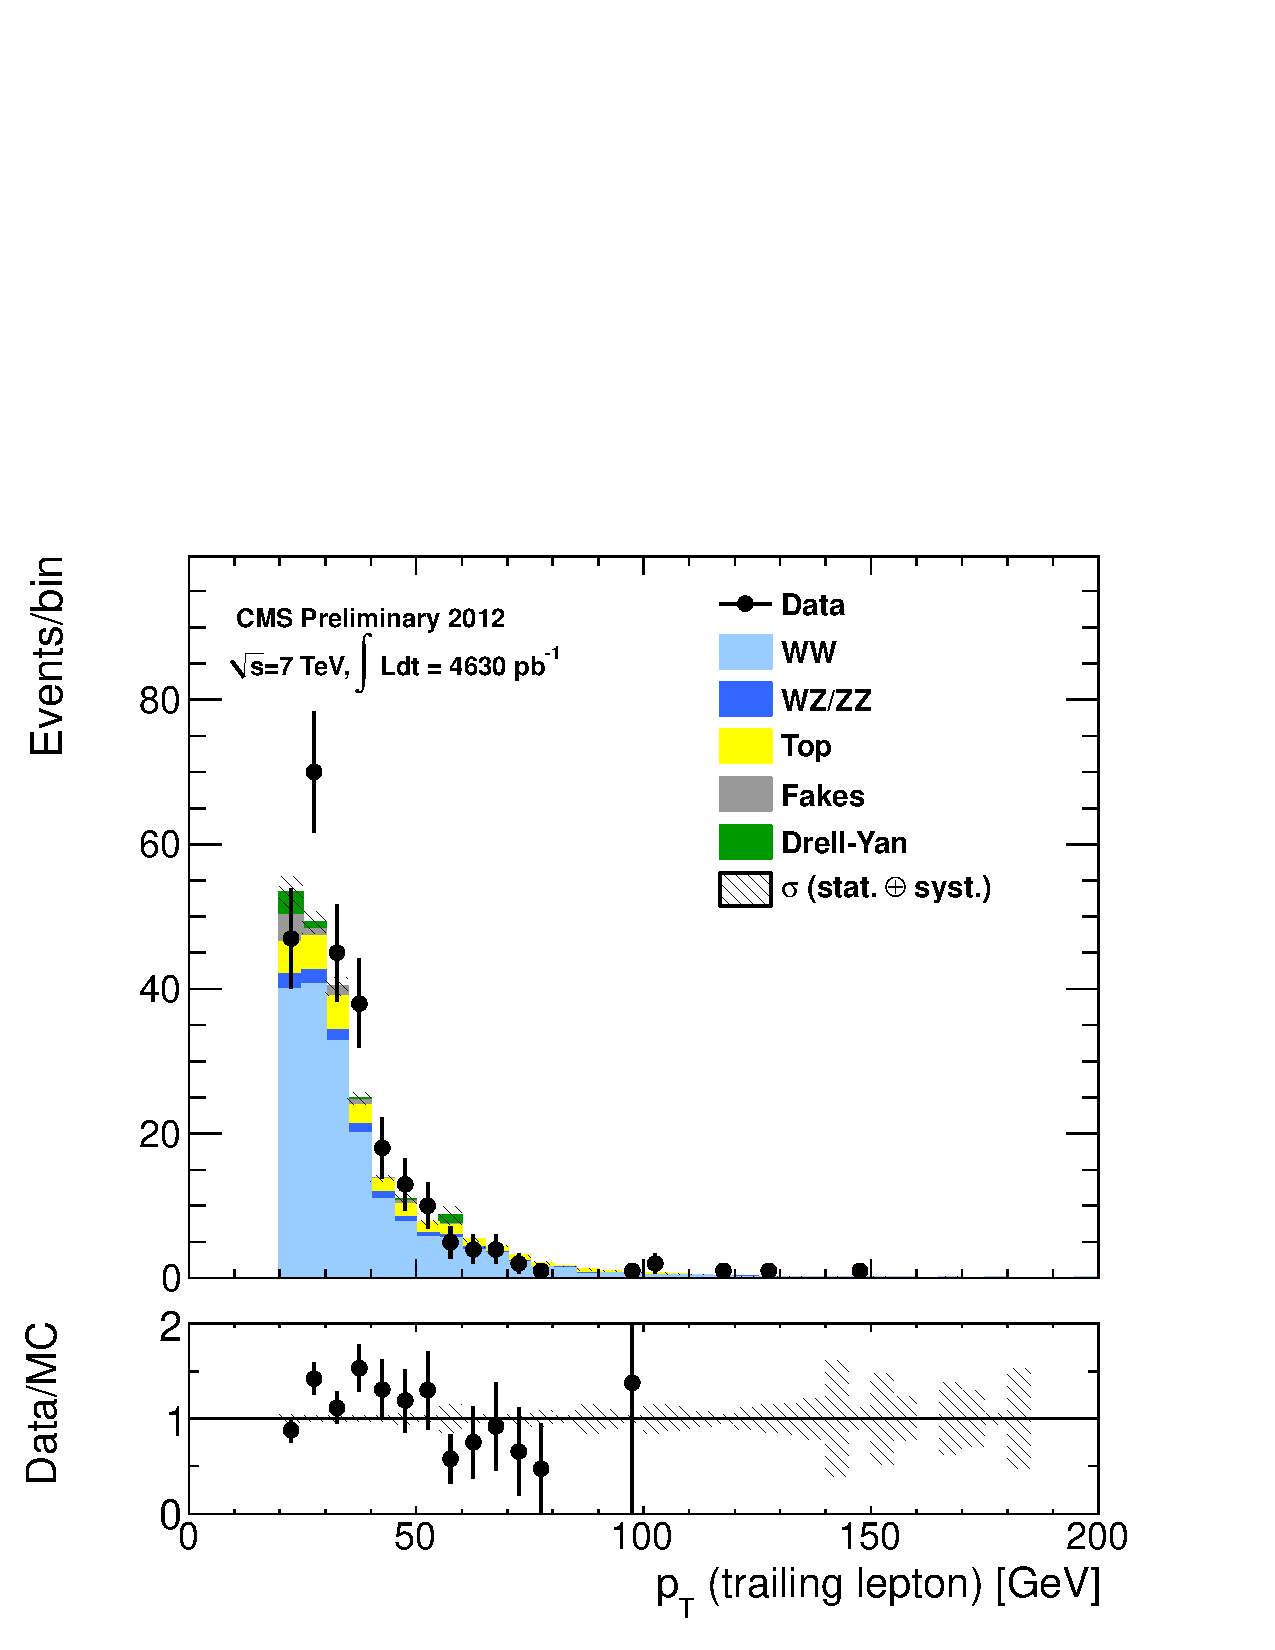
\includegraphics[width=.45\textwidth]{figures/pas_pt2_mm.pdf}}
\subfigure[Dilepton system $p_{T}$]{\label{subfig:fig_mmplots_ptll}
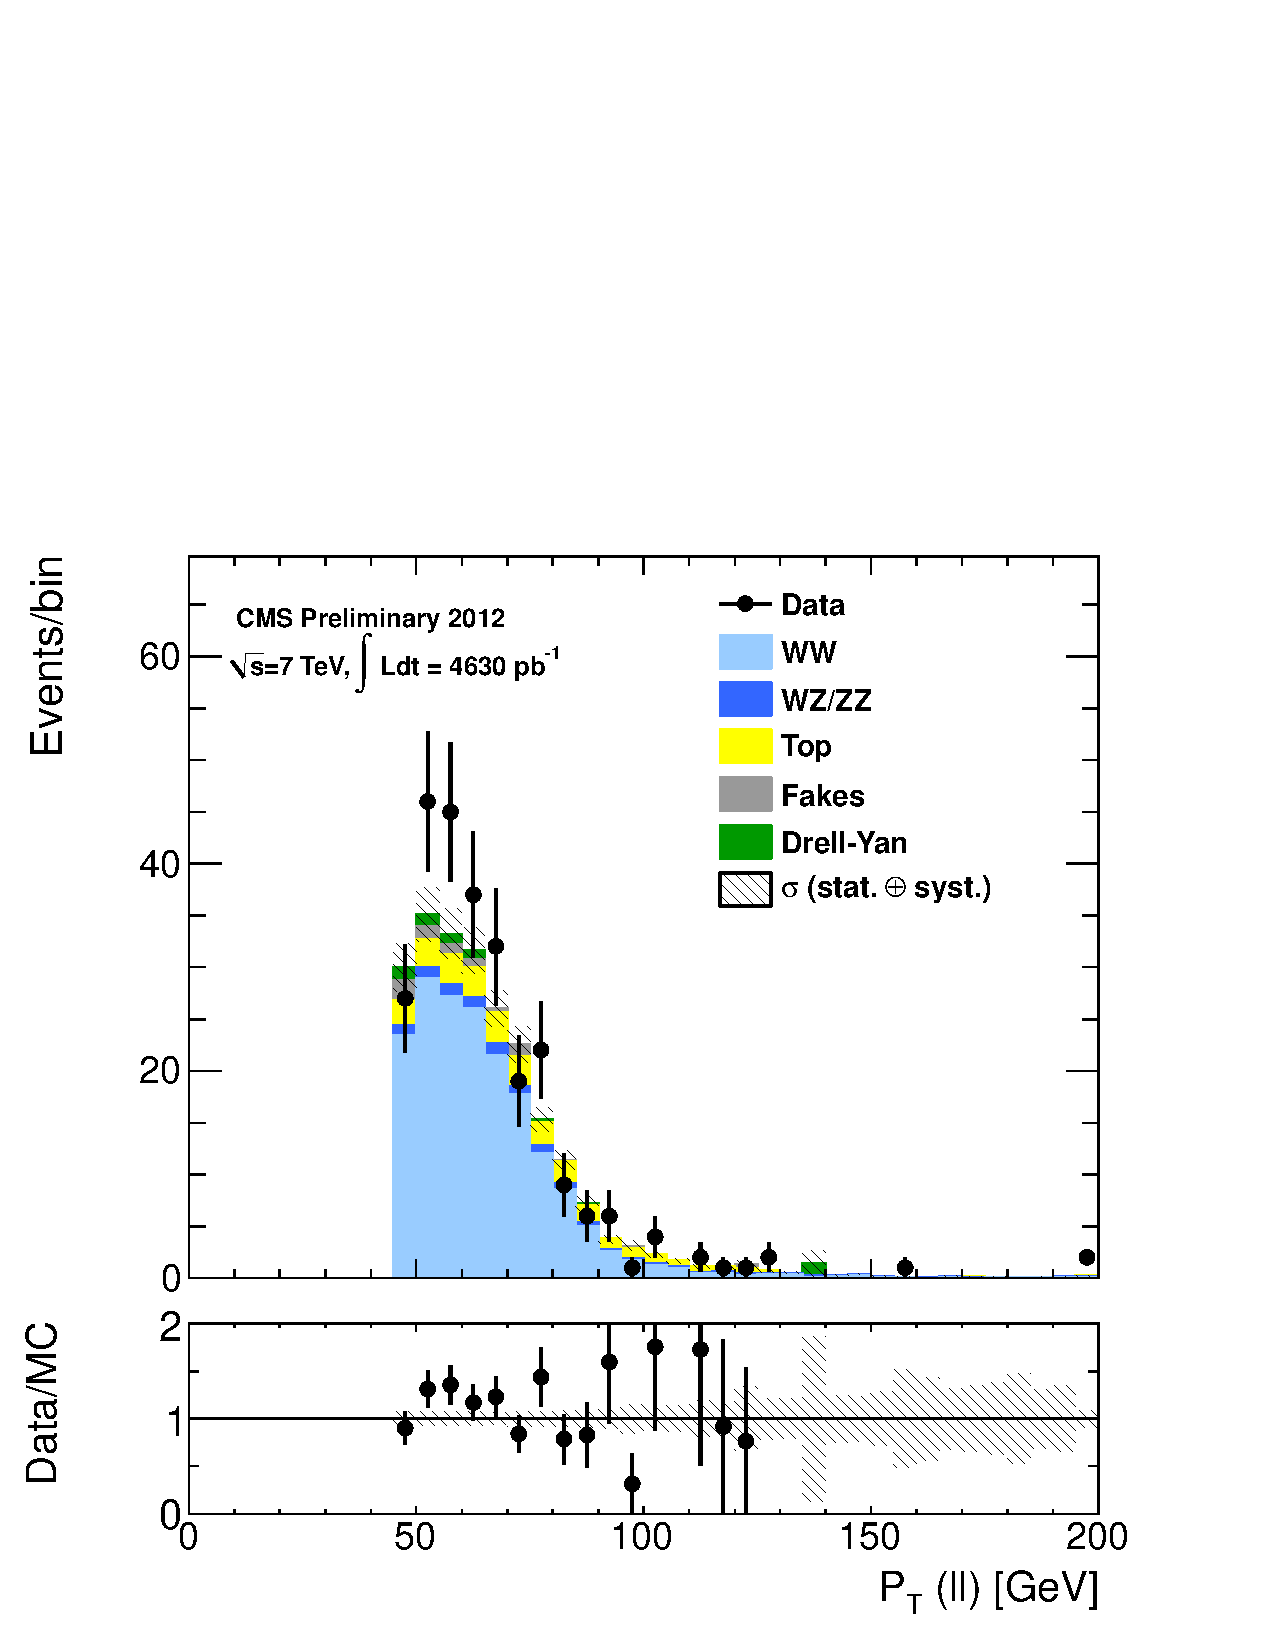
\includegraphics[width=.45\textwidth]{figures/pas_ptll_mm.pdf}}
\subfigure[Dilepton system invariant mass]{\label{subfig:fig_mmplots_M}
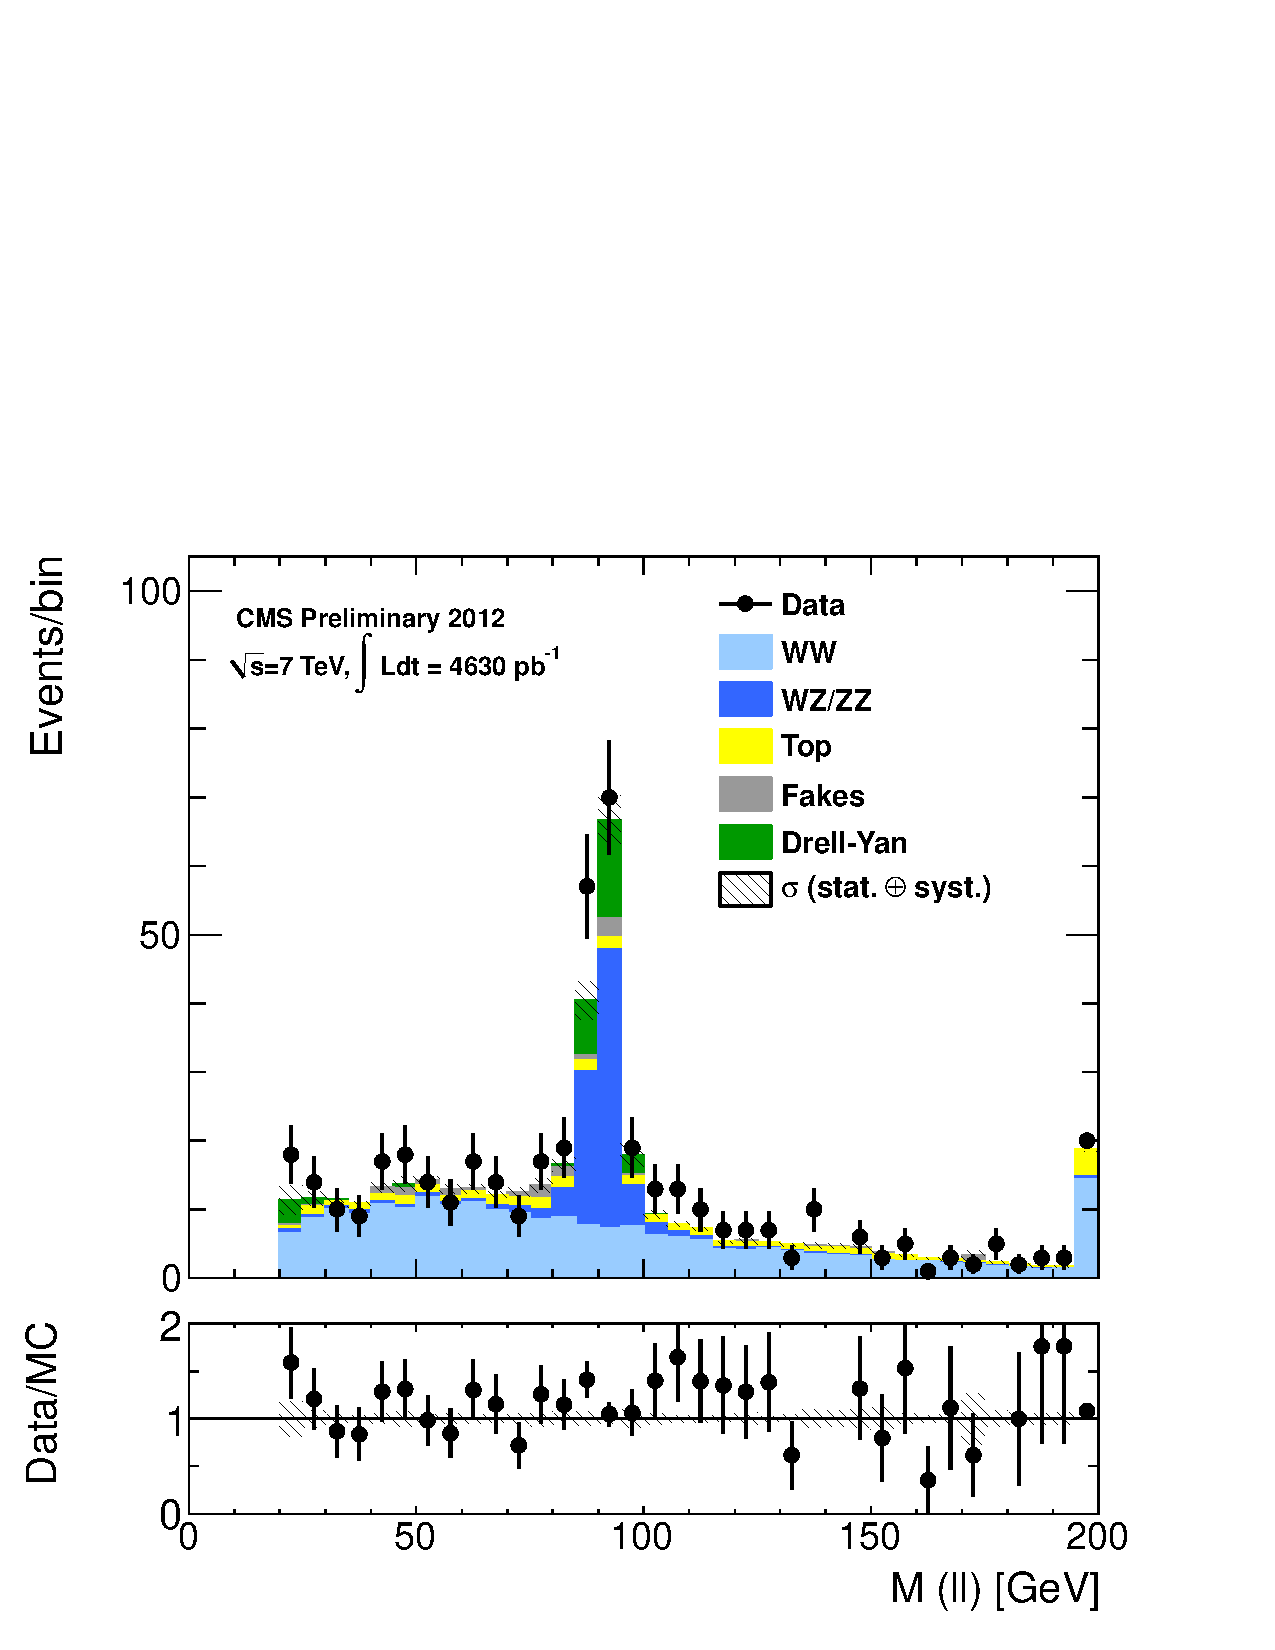
\includegraphics[width=.45\textwidth]{figures/pas_mll_mm.pdf}}
\caption{Kinematic distributions for expected and observed events in the $\mu\mu$ final state.
The dilepton system invariant mass distribution has the $Z$ mass veto relaxed.
The uncertainty on the expected events includes both statistical and systematic components.}
\label{fig:mmplots}
\end{center}
\end{figure}
%%%%%%%%

%
%
%
\clearpage
\subsection{$\mu e$ Channel}

The number of events observed and the background predictions and their uncertainties are
given in Table \ref{tab:data_yields_me}.
The distributions of the $p_{T}$ of the leading and trailing leptons, and the dilepton $p_{T}$
and invariant mass are shown in Figure \ref{fig:meplots}.
The signal efficiency,  $\varepsilon = 0.00979 \pm 0.00069~\mathrm{(syst.)}$.
The statistical uncertainty on the signal efficiency is negligible.
We obtain the following $WW$ cross-section measurement:

\begin{equation*}
\sigma_{WW}  = 53.45 \pm 3.75~\mathrm{(stat.)} \pm 4.01~\mathrm{(syst.)} \pm 2.41~\mathrm{(lumi.)~pb}. 
\end{equation*}

\begin{table}[ht!]
  \begin{center}
  \begin{tabular} {|c|c|}
\hline
Sample                & Yield $\pm$ stat $\pm$ syst \\ \hline \hline
$qqWW$                & 210.8 $\pm$  2.2 $\pm$ 13.3  \\ \hline
$ggWW$                & 12.8 $\pm$  0.3 $\pm$  3.9  \\ \hline
$t\bar{t} + tW$      & 38.1 $\pm$  1.3 $\pm$  7.1  \\ \hline
$W+jets$              & 15.4 $\pm$  1.8 $\pm$  5.5  \\ \hline
$WZ$/$ZZ$             &  4.2 $\pm$  0.1 $\pm$  0.4  \\ \hline
$Z/\gamma*$          &  0.0 $\pm$  0.0 $\pm$  0.0  \\ \hline
$W\gamma*/W+\gamma$ &  6.8 $\pm$  2.7 $\pm$  1.5  \\ \hline \hline
Total Bkgd.           & 64.7 $\pm$  3.1 $\pm$  5.8  \\ \hline \hline
Total Bkgd.+Signal    & 288.3 $\pm$  3.9 $\pm$ 15.0  \\ \hline \hline
Data                  & 319 \\ \hline
\end{tabular}
  \caption{Expected number of signal and background events from the data-driven methods for
  an integrated luminosity of \intlumi after applying the selection requirements in the $\mu e$ channel.}
   \label{tab:data_yields_me}
  \end{center}
\end{table}

%%%%%%%%
\begin{figure}[!hbtp]
\begin{center}
\subfigure[Leading lepton $p_{T}$]{\label{subfig:fig_meplots_pt1}
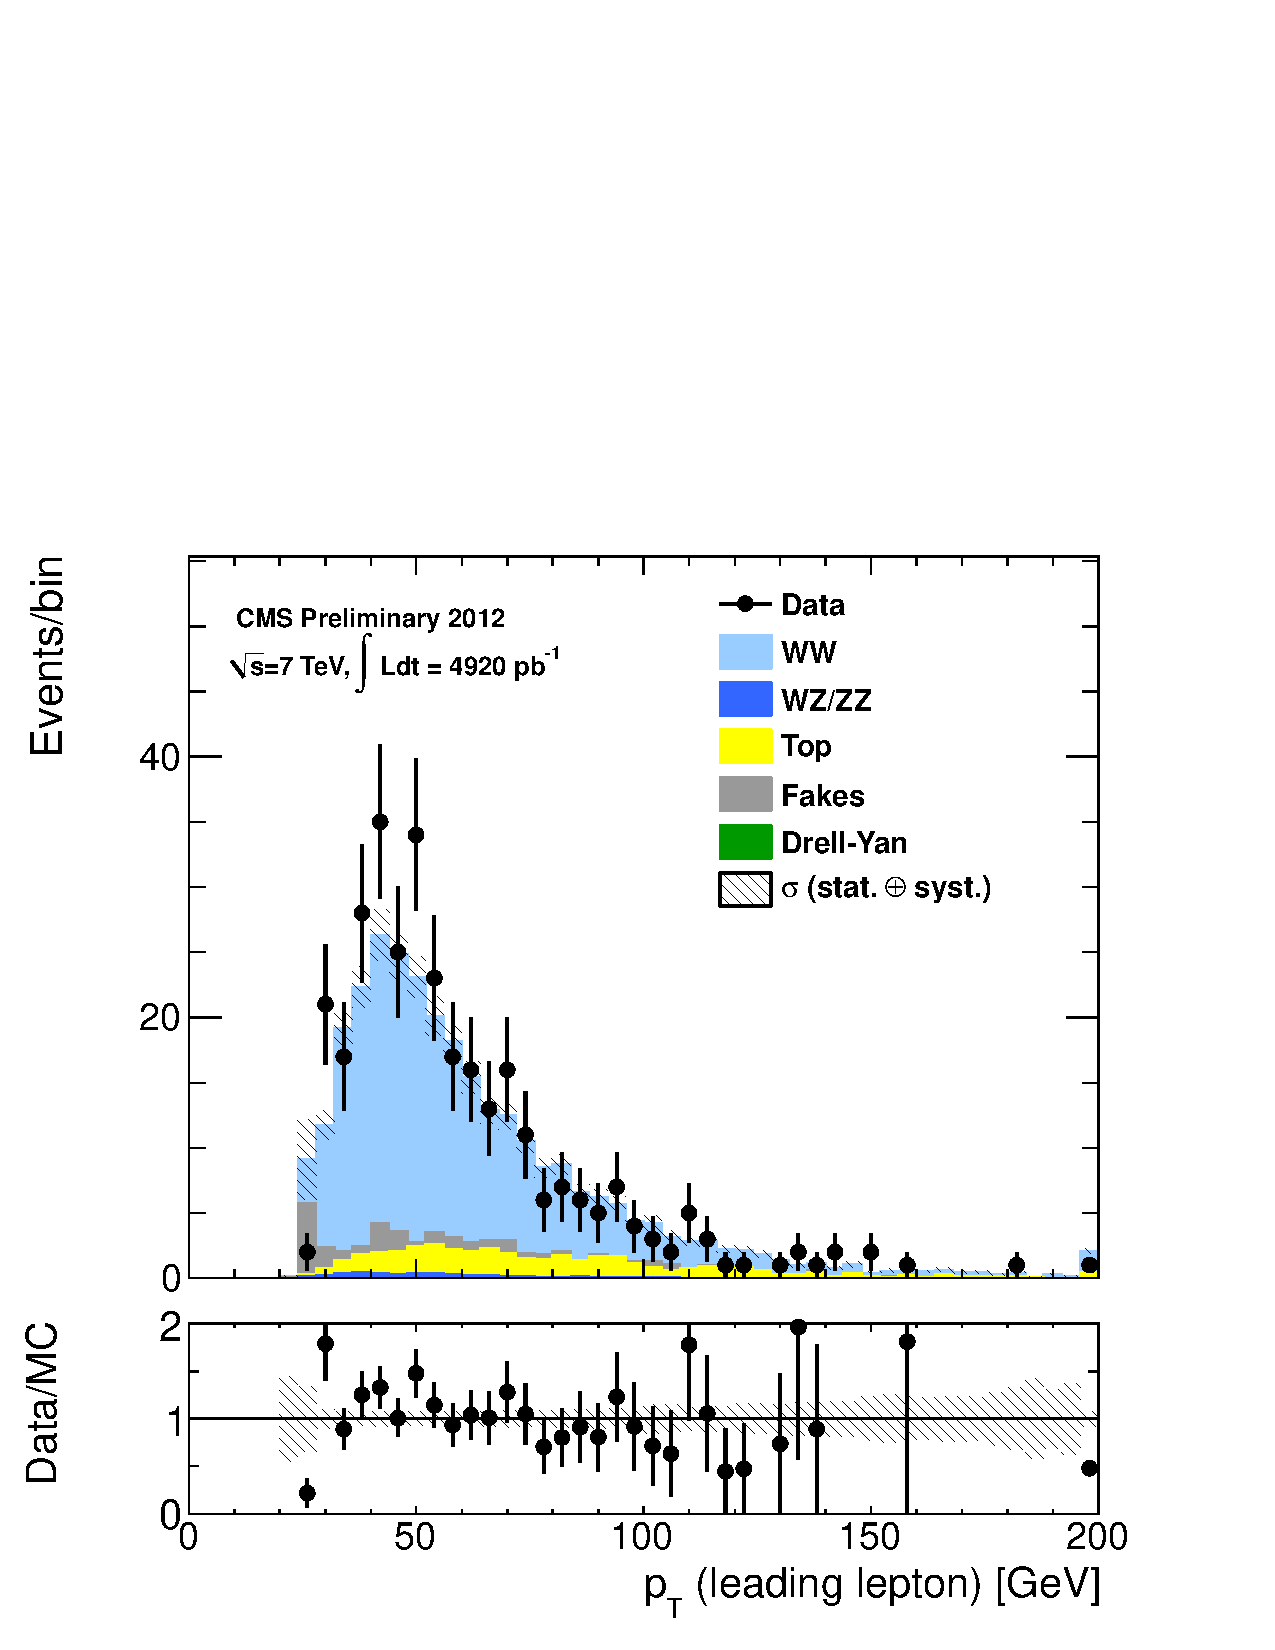
\includegraphics[width=.45\textwidth]{figures/pas_pt1_me.pdf}}
\subfigure[Trailing lepton $p_{T}$]{\label{subfig:fig_meplots_pt2}
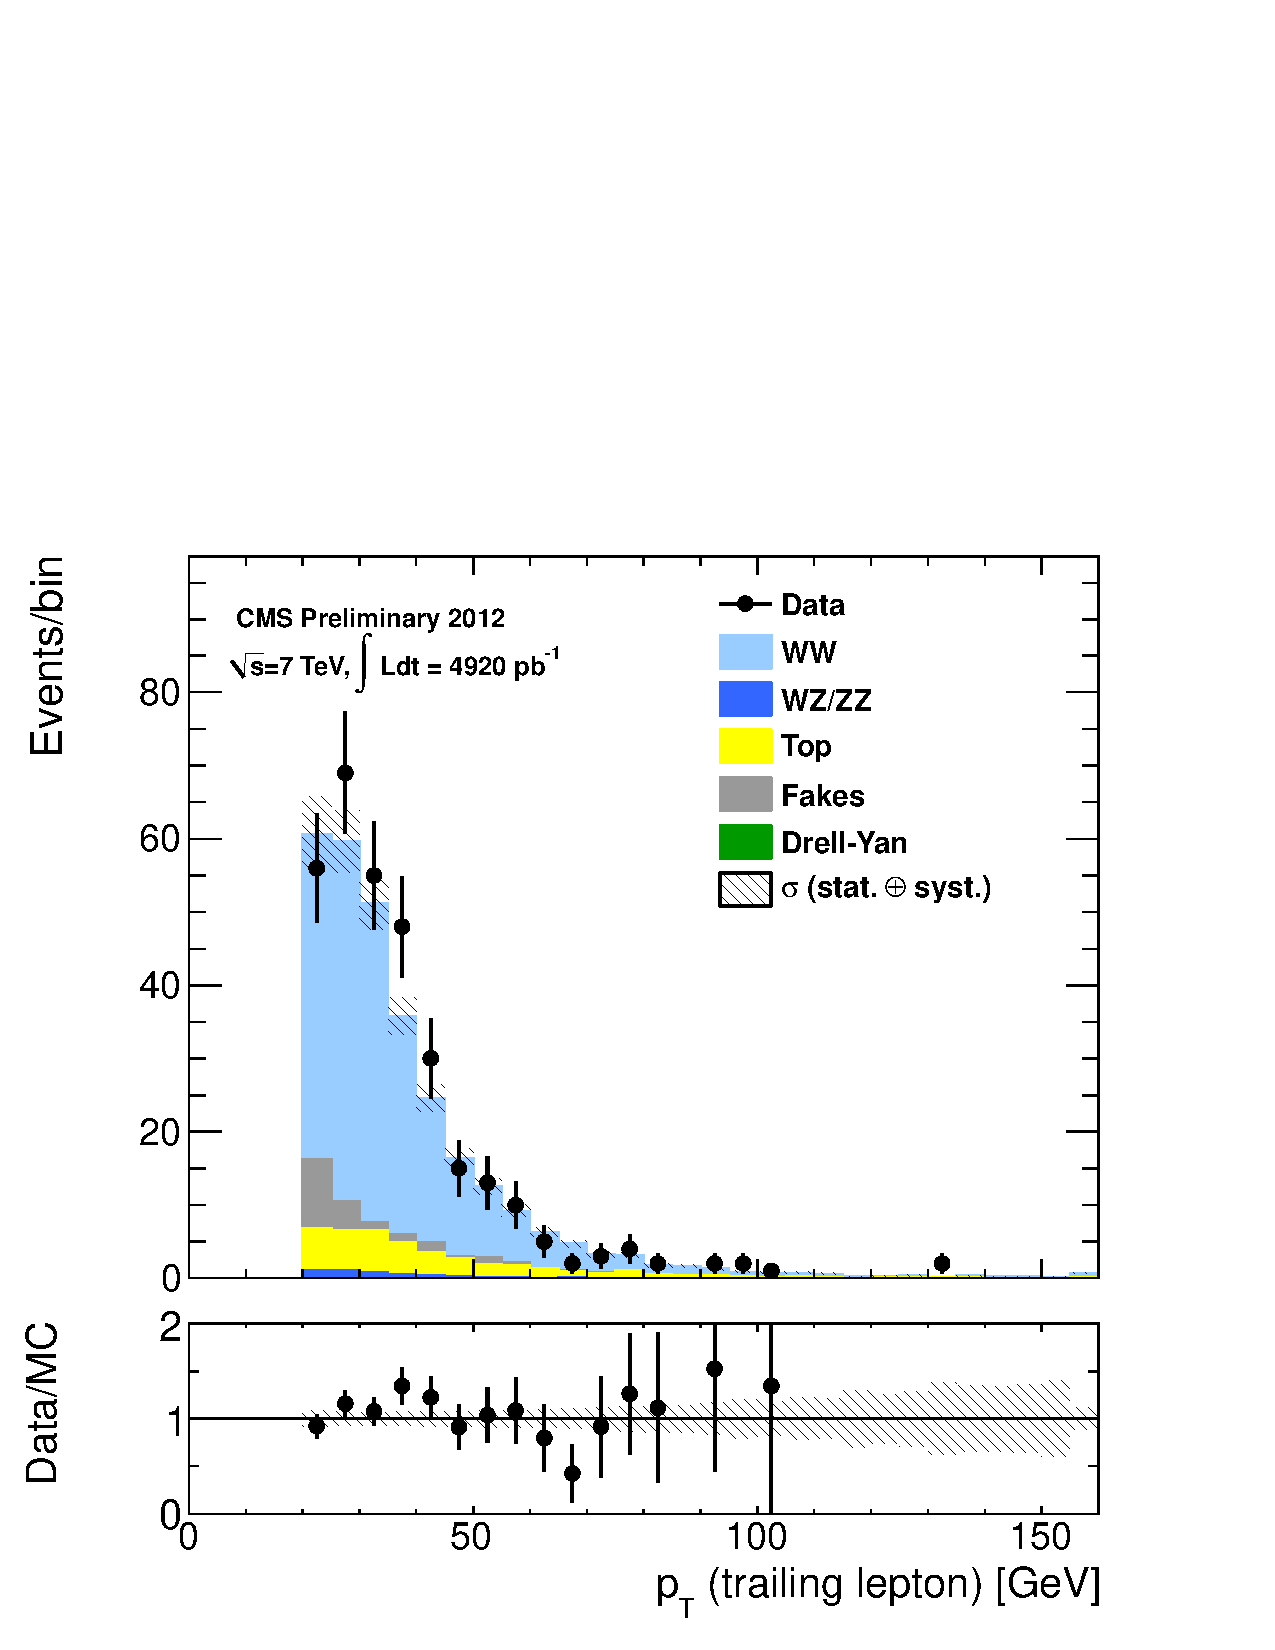
\includegraphics[width=.45\textwidth]{figures/pas_pt2_me.pdf}}
\subfigure[Dilepton system $p_{T}$]{\label{subfig:fig_meplots_ptll}
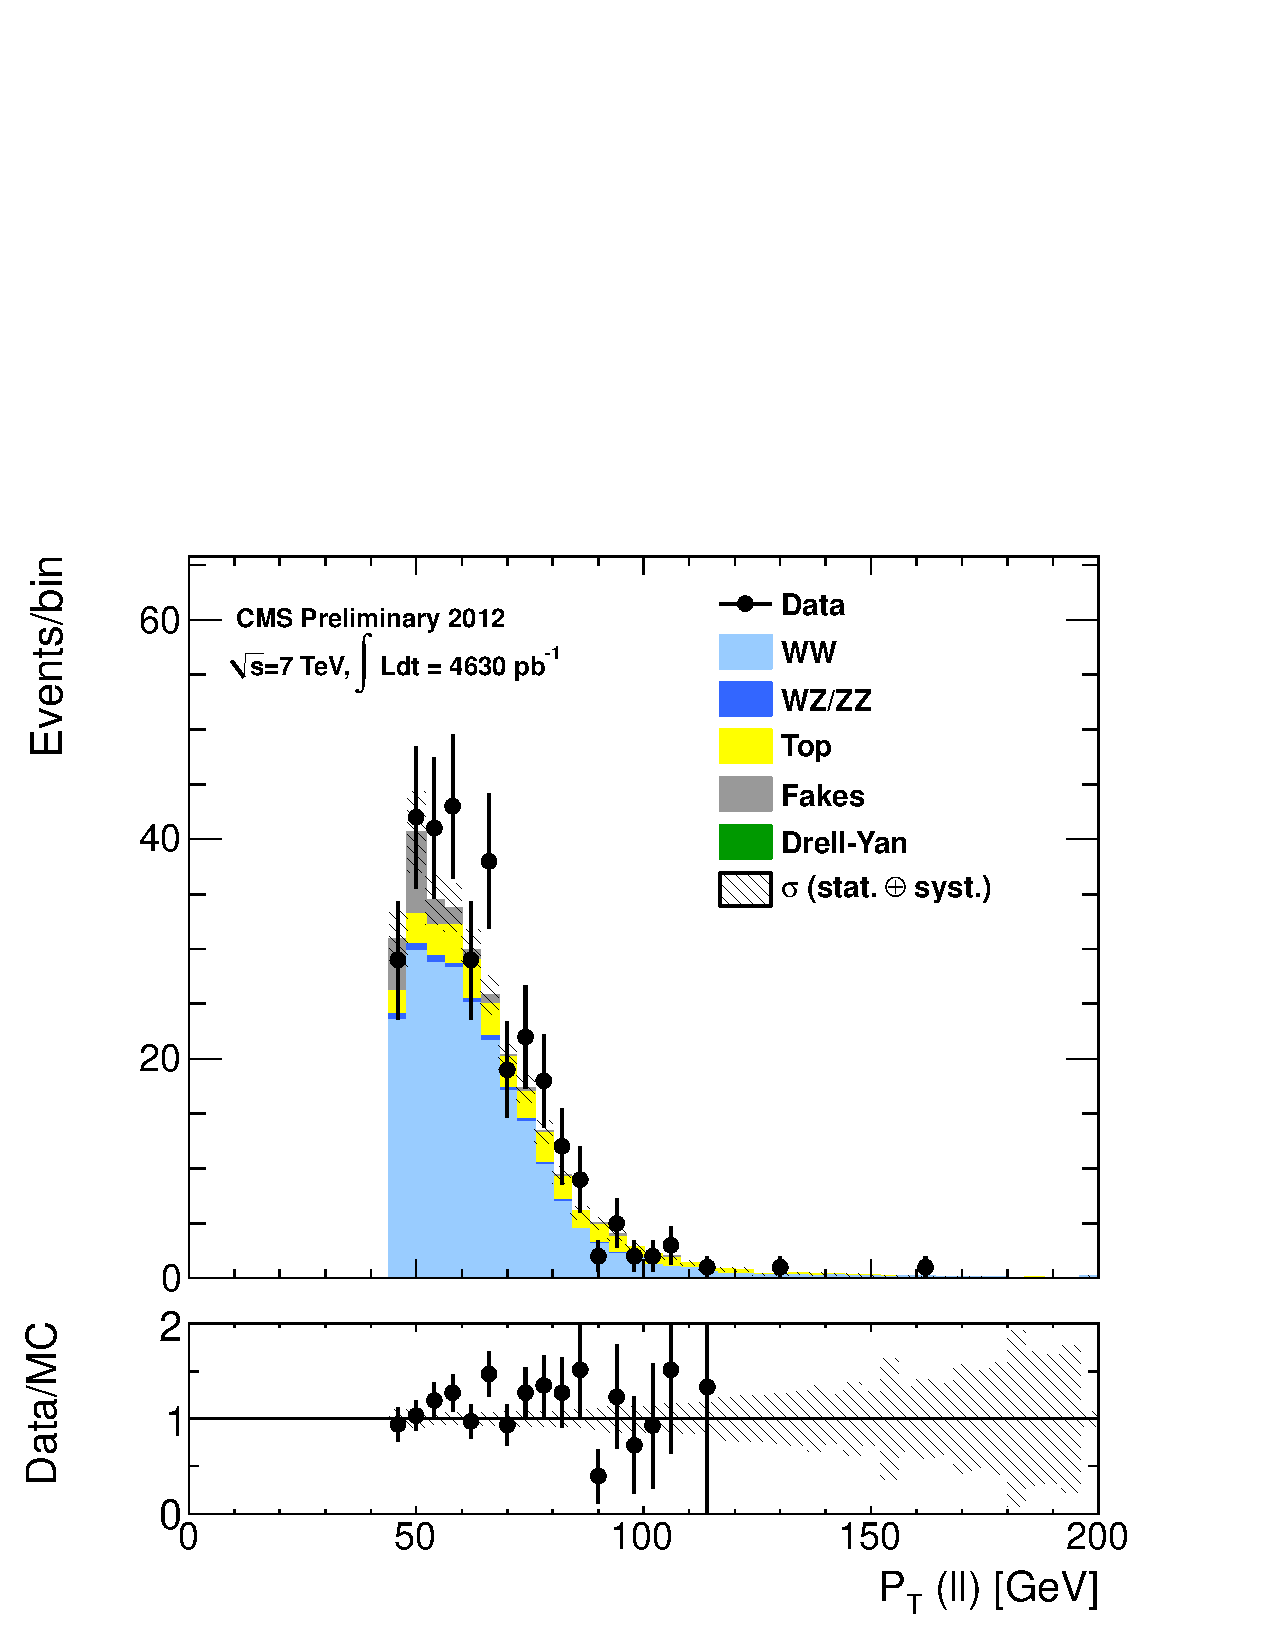
\includegraphics[width=.45\textwidth]{figures/pas_ptll_me.pdf}}
\subfigure[Dilepton system invariant mass]{\label{subfig:fig_meplots_M}
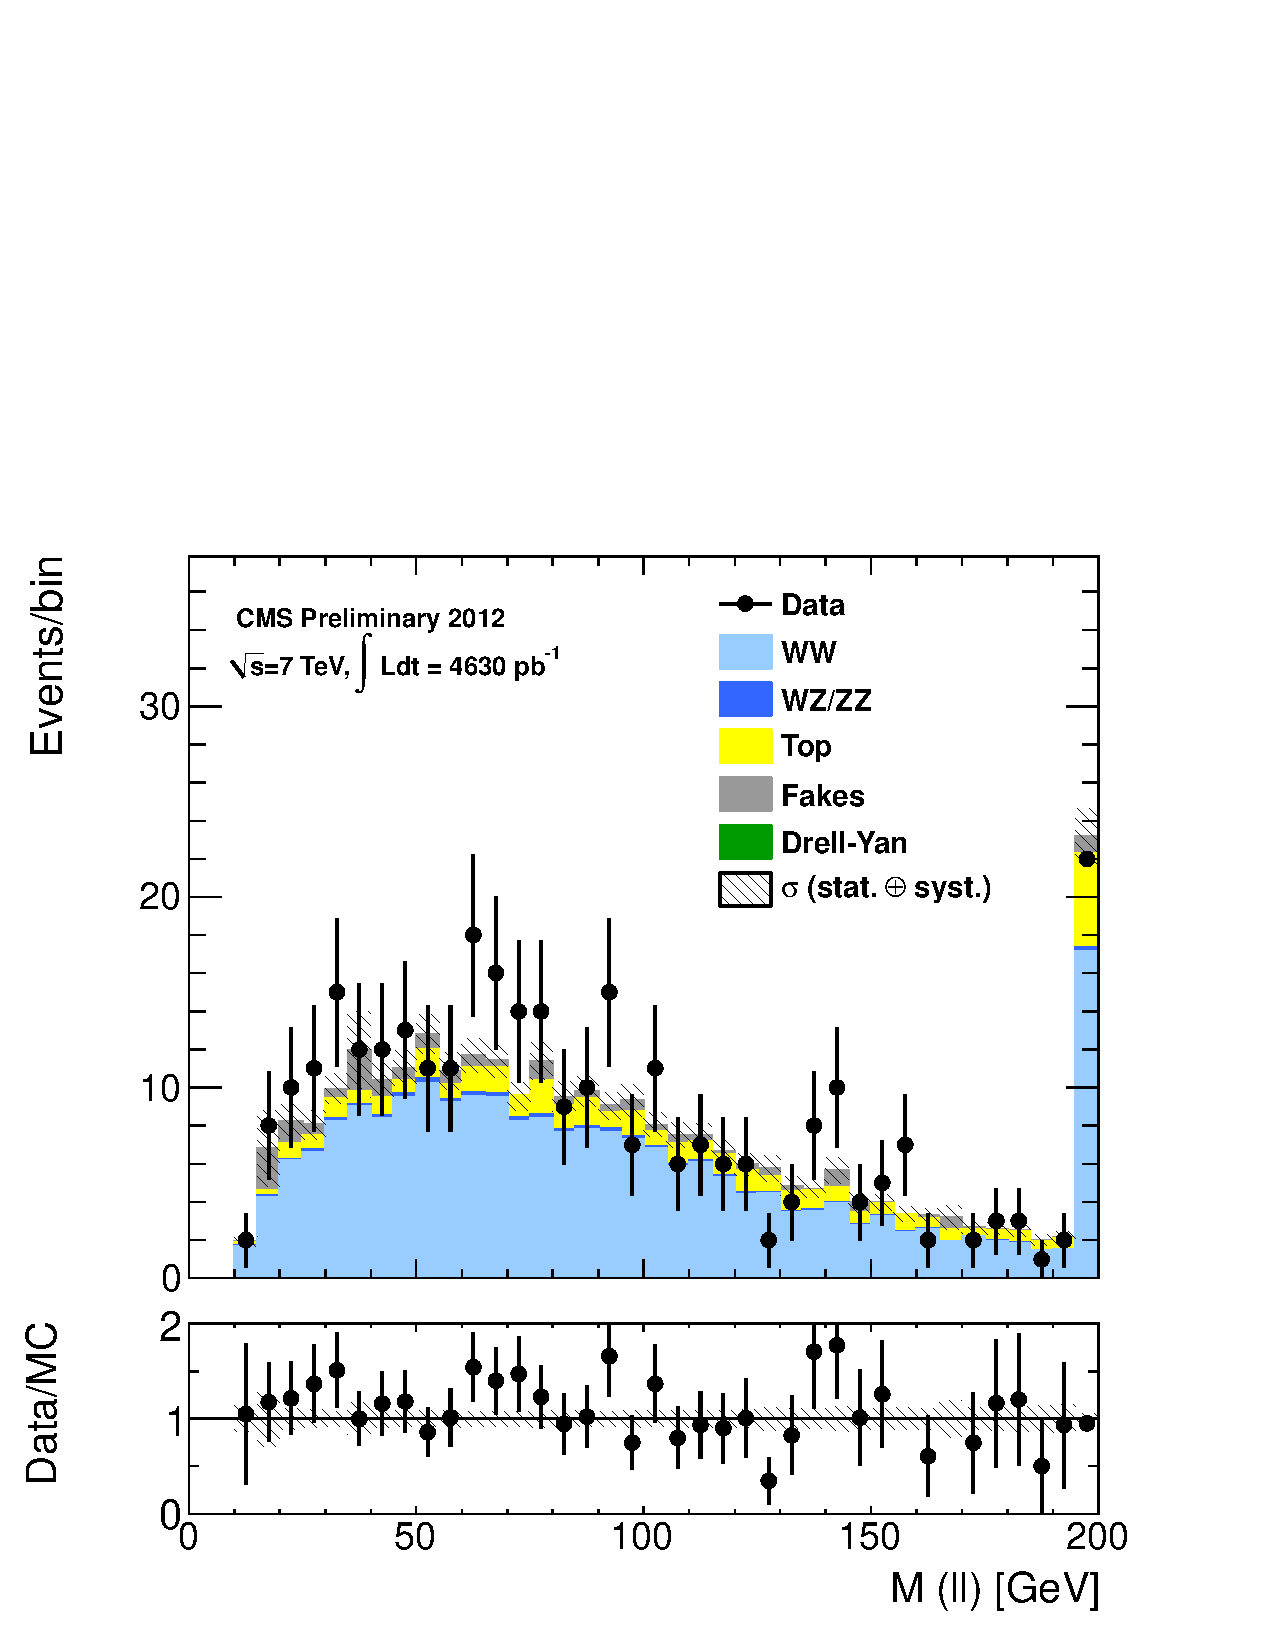
\includegraphics[width=.45\textwidth]{figures/pas_mll_me.pdf}}
\caption{Kinematic distributions for expected and observed events in the $\mu{e}$ final state.
The dilepton system invariant mass distribution has the $Z$ mass veto relaxed.
The uncertainty on the expected events includes both statistical and systematic components.}
\label{fig:meplots}
\end{center}
\end{figure}
%%%%%%%%

%
%
%
\clearpage
\subsection{$e \mu$ Channel}

The number of events observed and the background predictions and their uncertainties are
given in Table \ref{tab:data_yields_em}.
The distributions of the $p_{T}$ of the leading and trailing leptons, and the dilepton $p_{T}$
and invariant mass are shown in Figure \ref{fig:emplots}.
The signal efficiency,  $\varepsilon = 0.01103 \pm 0.00078~\mathrm{(syst.)}$.
The statistical uncertainty on the signal efficiency is negligible.
We obtain the following $WW$ cross-section measurement:

\begin{equation*}
\sigma_{WW}  = 49.54 \pm 3.48~\mathrm{(stat.)} \pm 4.28~\mathrm{(syst.)} \pm 2.23~\mathrm{(lumi.)~pb}. 
\end{equation*}

\begin{table}[ht!]
  \begin{center}
  \begin{tabular} {|c|c|}
\hline
Sample                & Yield $\pm$ stat $\pm$ syst \\ \hline \hline
$qqWW$                & 238.3 $\pm$  2.4 $\pm$ 15.0  \\ \hline
$ggWW$                & 13.8 $\pm$  0.3 $\pm$  4.2  \\ \hline
$t\bar{t} + tW$      & 42.1 $\pm$  1.3 $\pm$  7.9  \\ \hline
$W+jets$              & 27.8 $\pm$  2.6 $\pm$ 10.0  \\ \hline
$WZ$/$ZZ$             &  6.1 $\pm$  0.2 $\pm$  0.6  \\ \hline
$Z/\gamma*$          &  0.0 $\pm$  0.0 $\pm$  0.0  \\ \hline
$W\gamma*/W+\gamma$ &  6.9 $\pm$  1.2 $\pm$  2.0  \\ \hline \hline
Total Bkgd.           & 83.3 $\pm$  3.2 $\pm$ 12.9  \\ \hline \hline
Total Bkgd.+Signal    & 335.4 $\pm$  4.0 $\pm$ 20.3  \\ \hline \hline
Data                  & 349 \\ \hline
\end{tabular}
  \caption{Expected number of signal and background events from the data-driven methods for
  an integrated luminosity of \intlumi after applying the selection requirements in the $e \mu$ channel.}
   \label{tab:data_yields_em}
  \end{center}
\end{table}

%%%%%%%%
\begin{figure}[!hbtp]
\begin{center}
\subfigure[Leading lepton $p_{T}$]{\label{subfig:fig_emplots_pt1}
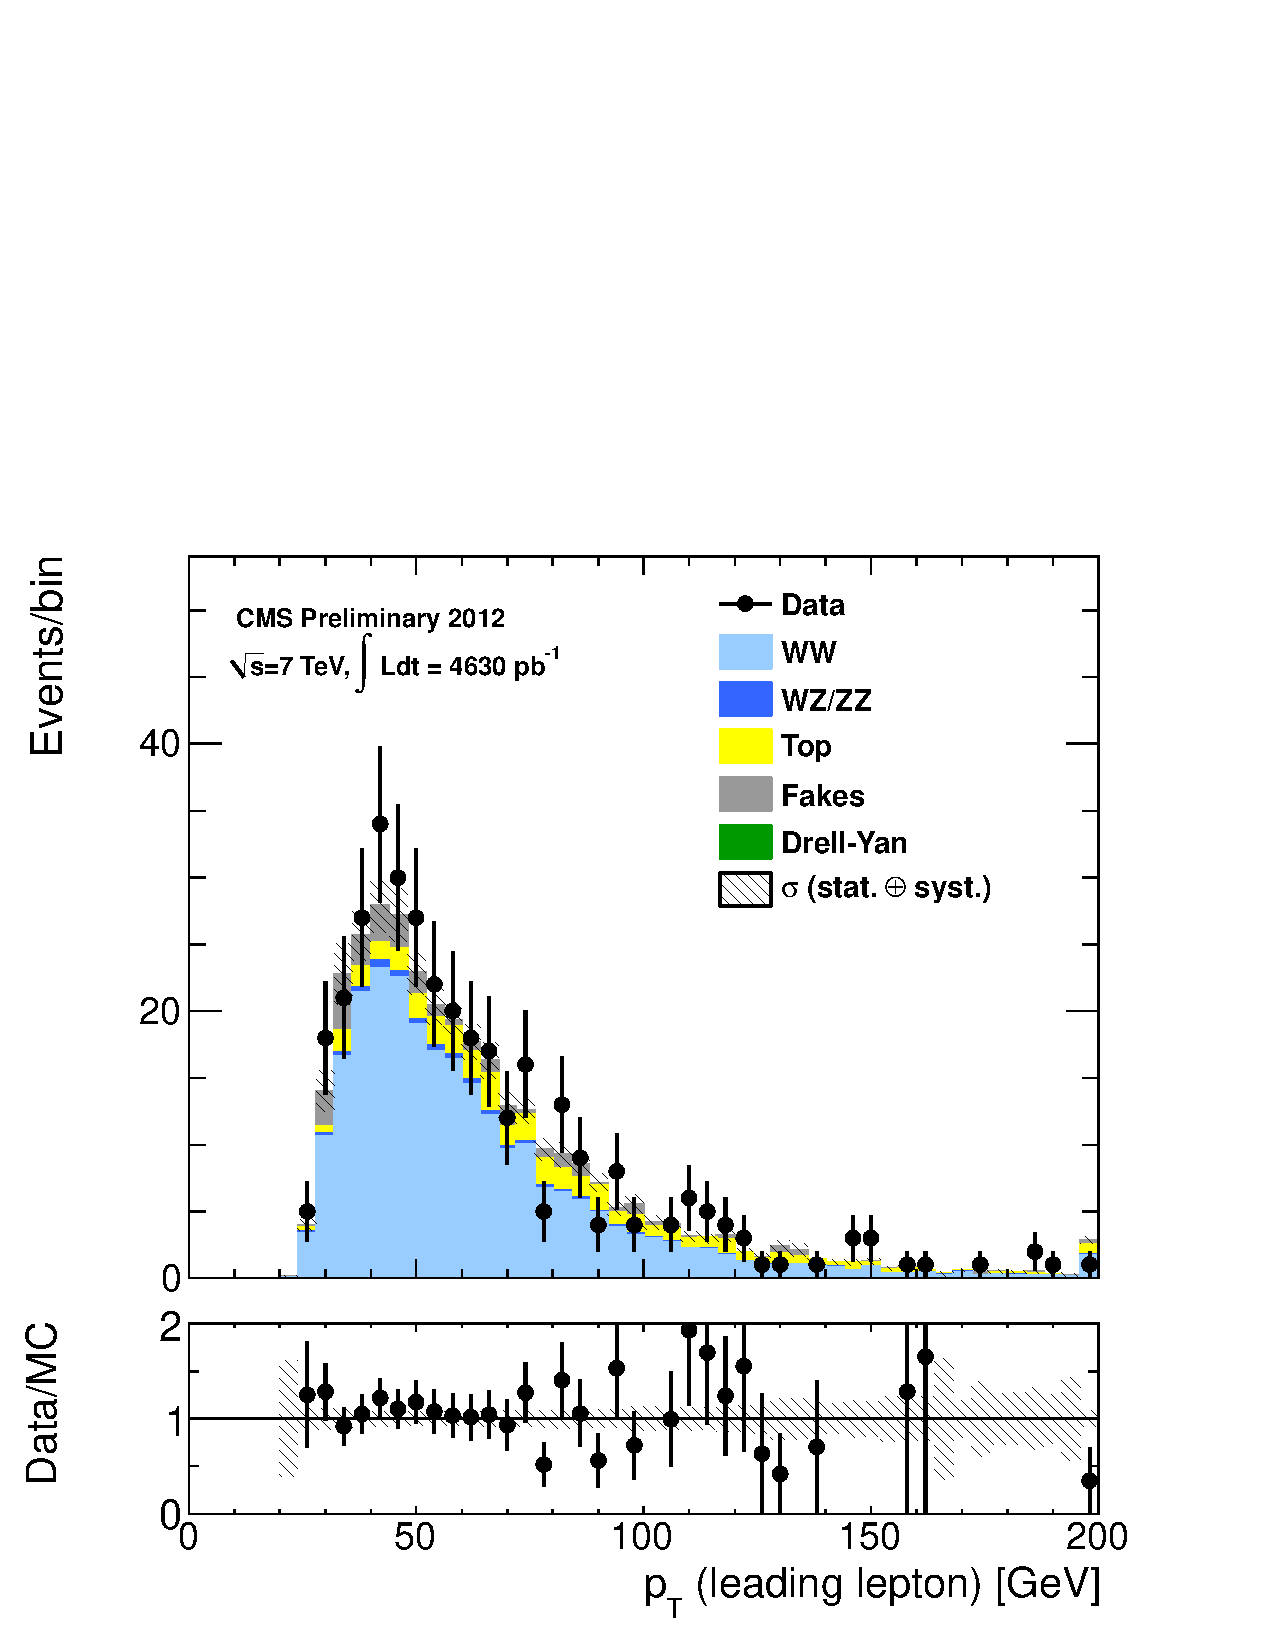
\includegraphics[width=.45\textwidth]{figures/pas_pt1_em.pdf}}
\subfigure[Trailing lepton $p_{T}$]{\label{subfig:fig_emplots_pt2}
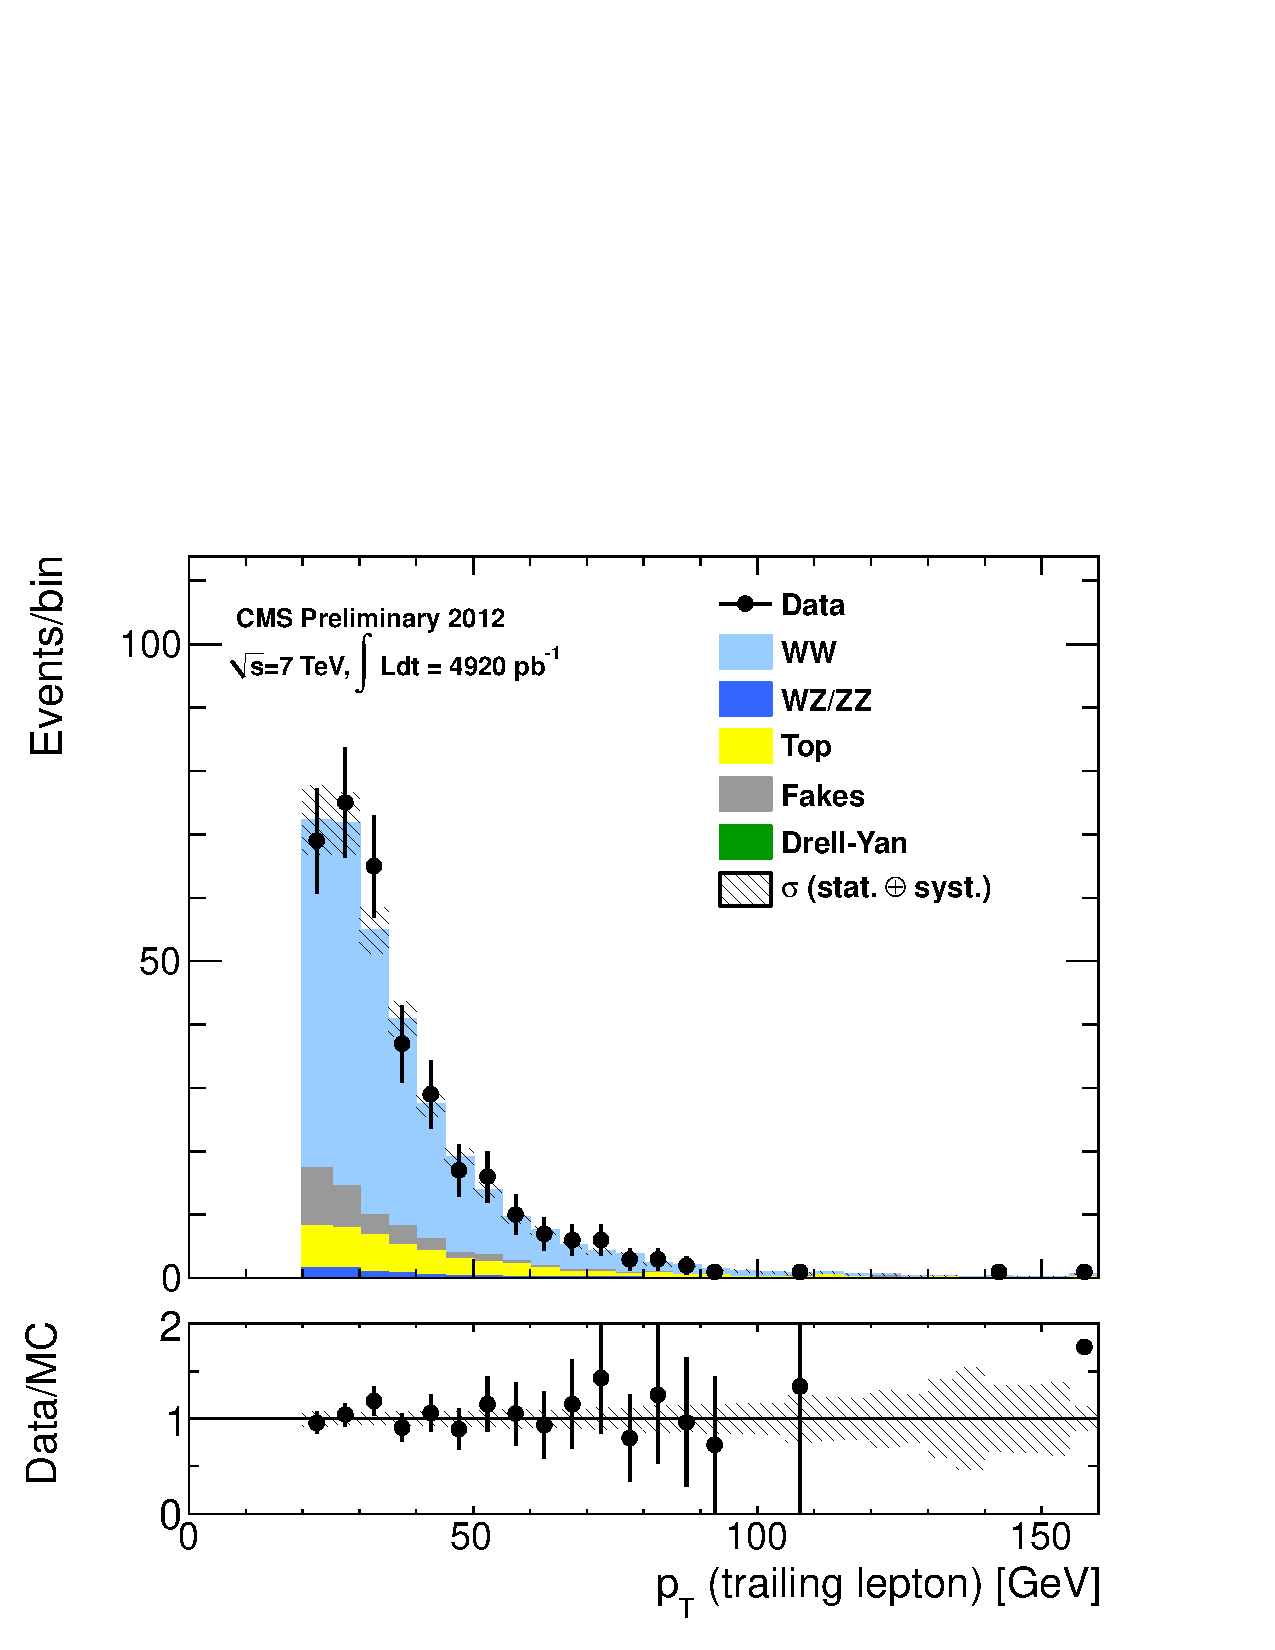
\includegraphics[width=.45\textwidth]{figures/pas_pt2_em.pdf}}
\subfigure[Dilepton system $p_{T}$]{\label{subfig:fig_emplots_ptll}
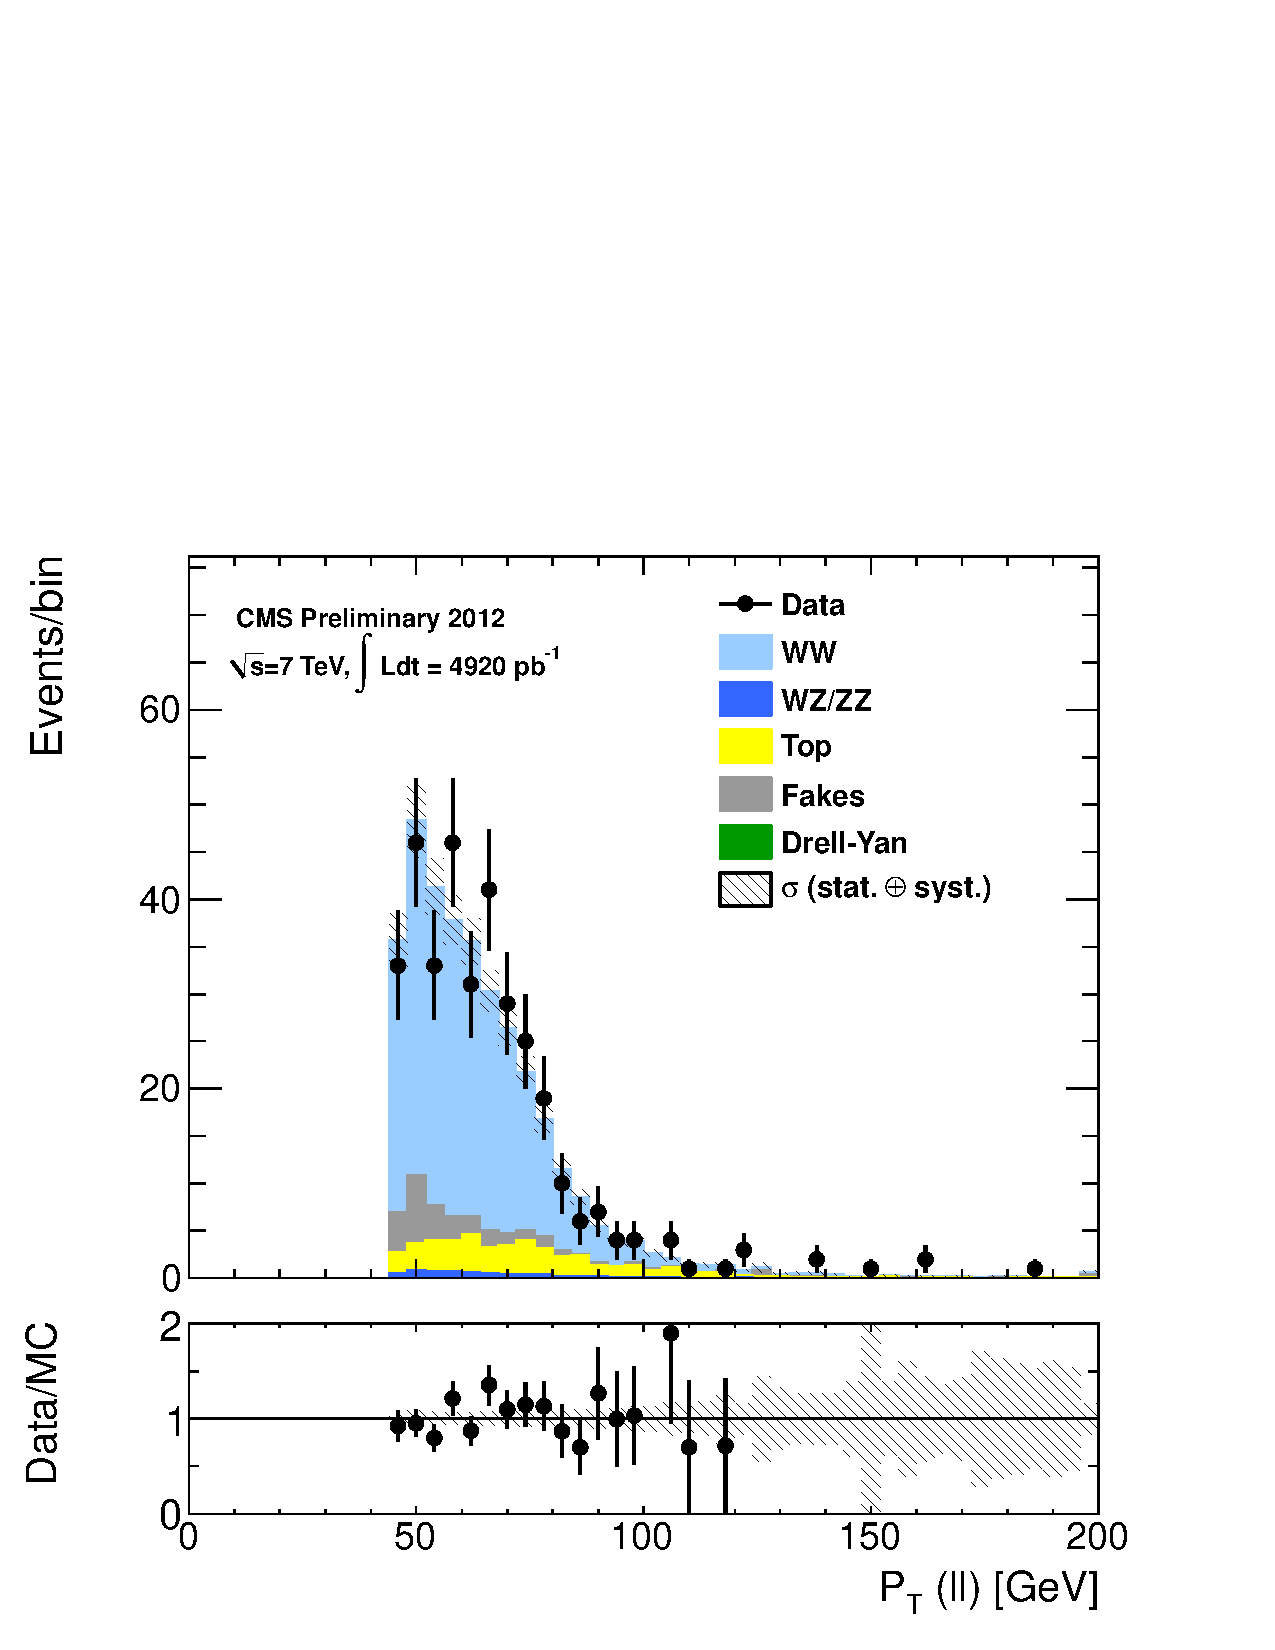
\includegraphics[width=.45\textwidth]{figures/pas_ptll_em.pdf}}
\subfigure[Dilepton system invariant mass]{\label{subfig:fig_emplots_M}
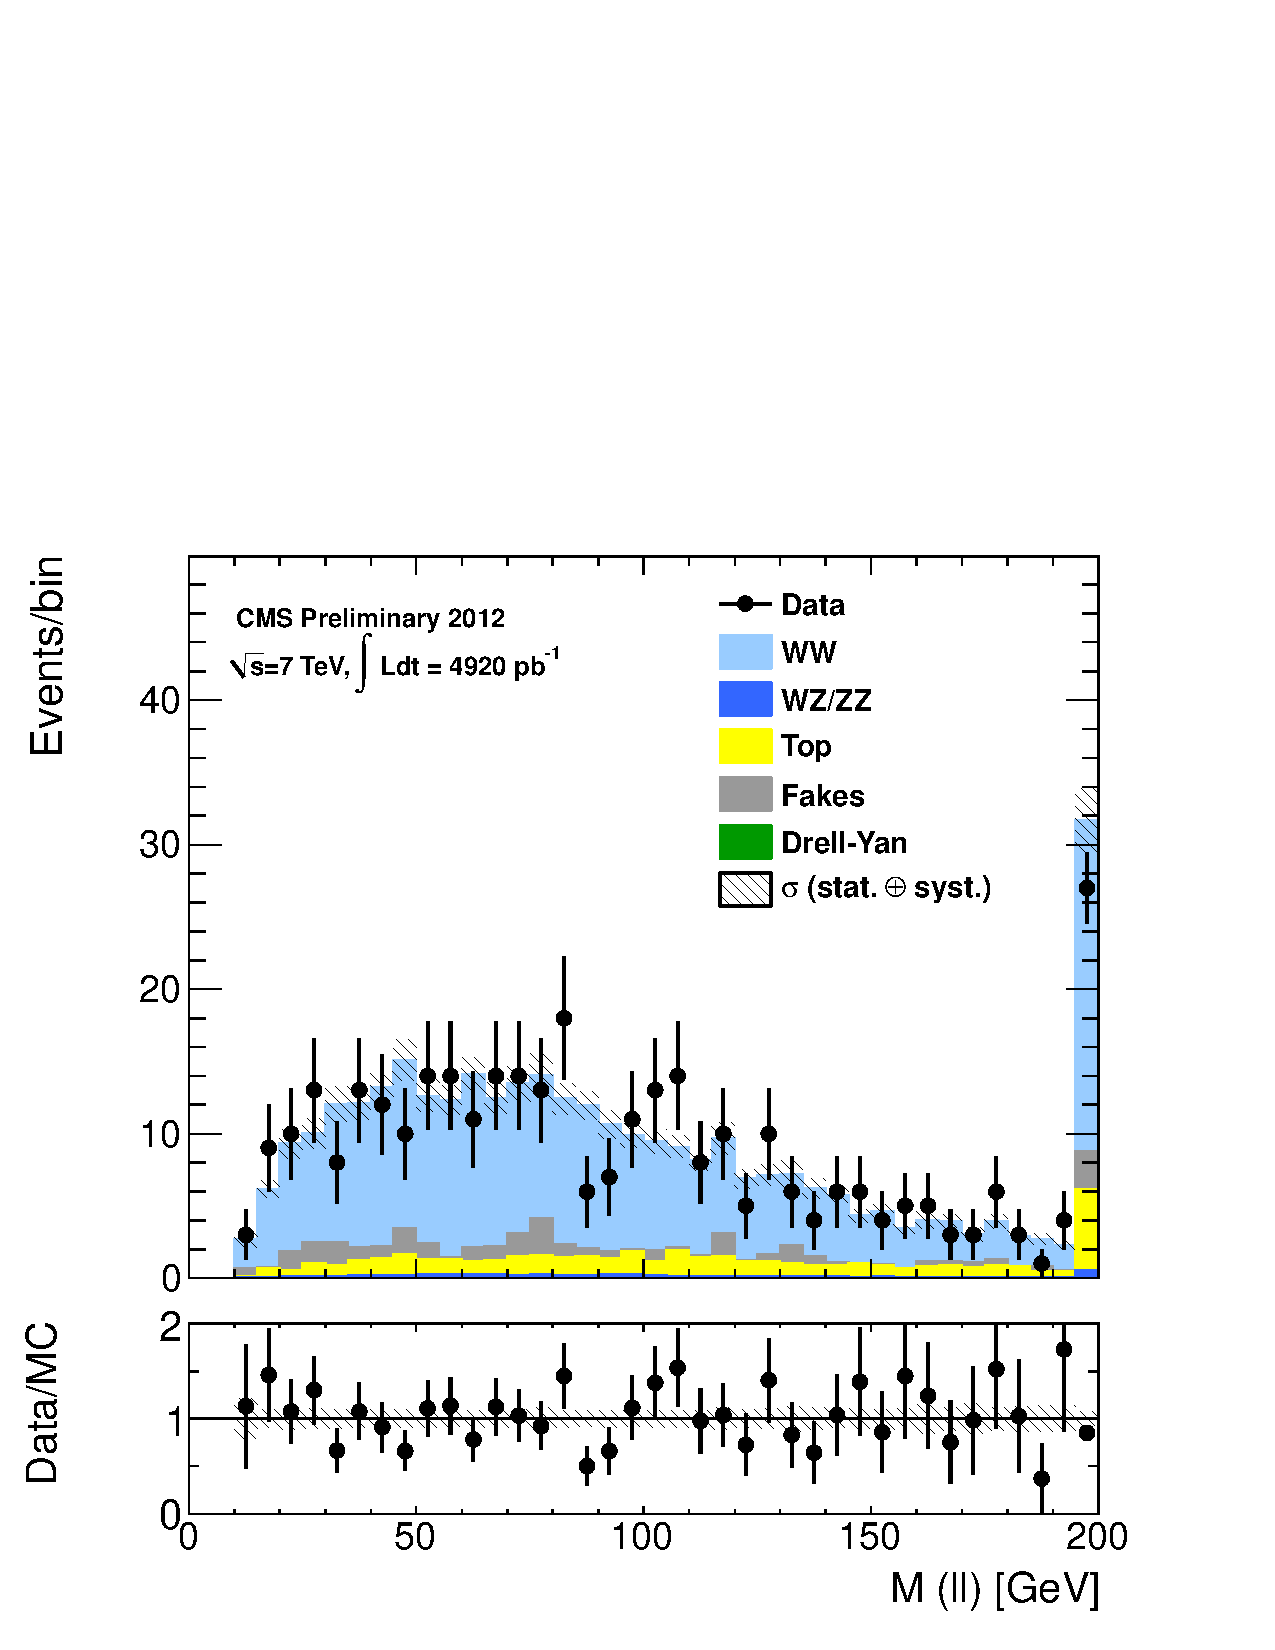
\includegraphics[width=.45\textwidth]{figures/pas_mll_em.pdf}}
\caption{Kinematic distributions for expected and observed events in the $e\mu$ final state.
The dilepton system invariant mass distribution has the $Z$ mass veto relaxed.
The uncertainty on the expected events includes both statistical and systematic components.}
\label{fig:emplots}
\end{center}
\end{figure}
%%%%%%%%

%
%
%
\clearpage
\subsection{$ee$ Channel}

The number of events observed and the background predictions and their uncertainties are
given in Table \ref{tab:data_yields_ee}.
The distributions of the $p_{T}$ of the leading and trailing leptons, and the dilepton $p_{T}$
and invariant mass are shown in Figure \ref{fig:eeplots}.
The signal efficiency,  $\varepsilon = 0.00507 \pm 0.00036~\mathrm{(syst.)}$.
The statistical uncertainty on the signal efficiency is negligible.
We obtain the following $WW$ cross-section measurement:

\begin{equation*}
\sigma_{WW}  = 62.76 \pm 5.72~\mathrm{(stat.)} \pm 5.16~\mathrm{(syst.)} \pm 2.82~\mathrm{(lumi.)~pb}.
\end{equation*}

\begin{table}[ht!]
  \begin{center}
  \begin{tabular} {|c|c|}
\hline
Sample                & Yield $\pm$ stat $\pm$ syst \\ \hline \hline
$qqWW$                & 109.2 $\pm$  1.6 $\pm$  6.9  \\ \hline
$ggWW$                &  6.7 $\pm$  0.2 $\pm$  2.0  \\ \hline
$t\bar{t} + tW$      & 16.8 $\pm$  0.8 $\pm$  3.1  \\ \hline
$W+jets$              & 10.2 $\pm$  1.1 $\pm$  3.7  \\ \hline
$WZ$/$ZZ$             &  6.5 $\pm$  0.2 $\pm$  0.5  \\ \hline
$Z/\gamma*$          &  7.0 $\pm$  2.7 $\pm$  3.0  \\ \hline
$W\gamma*/W+\gamma$ &  3.7 $\pm$  1.0 $\pm$  1.0  \\ \hline \hline
Total Bkgd.           & 44.2 $\pm$  3.1 $\pm$  5.8  \\ \hline \hline
Total Bkgd.+Signal    & 160.1 $\pm$  3.5 $\pm$  9.2  \\ \hline \hline
Data                  & 199 \\ \hline
\end{tabular}
  \caption{Expected number of signal and background events from the data-driven methods for
  an integrated luminosity of \intlumi after applying the selection requirements in the $ee$ channel.}
   \label{tab:data_yields_ee}
  \end{center}
\end{table}

%%%%%%%%
\begin{figure}[!hbtp]
\begin{center}
\subfigure[Leading lepton $p_{T}$]{\label{subfig:fig_eeplots_pt1}
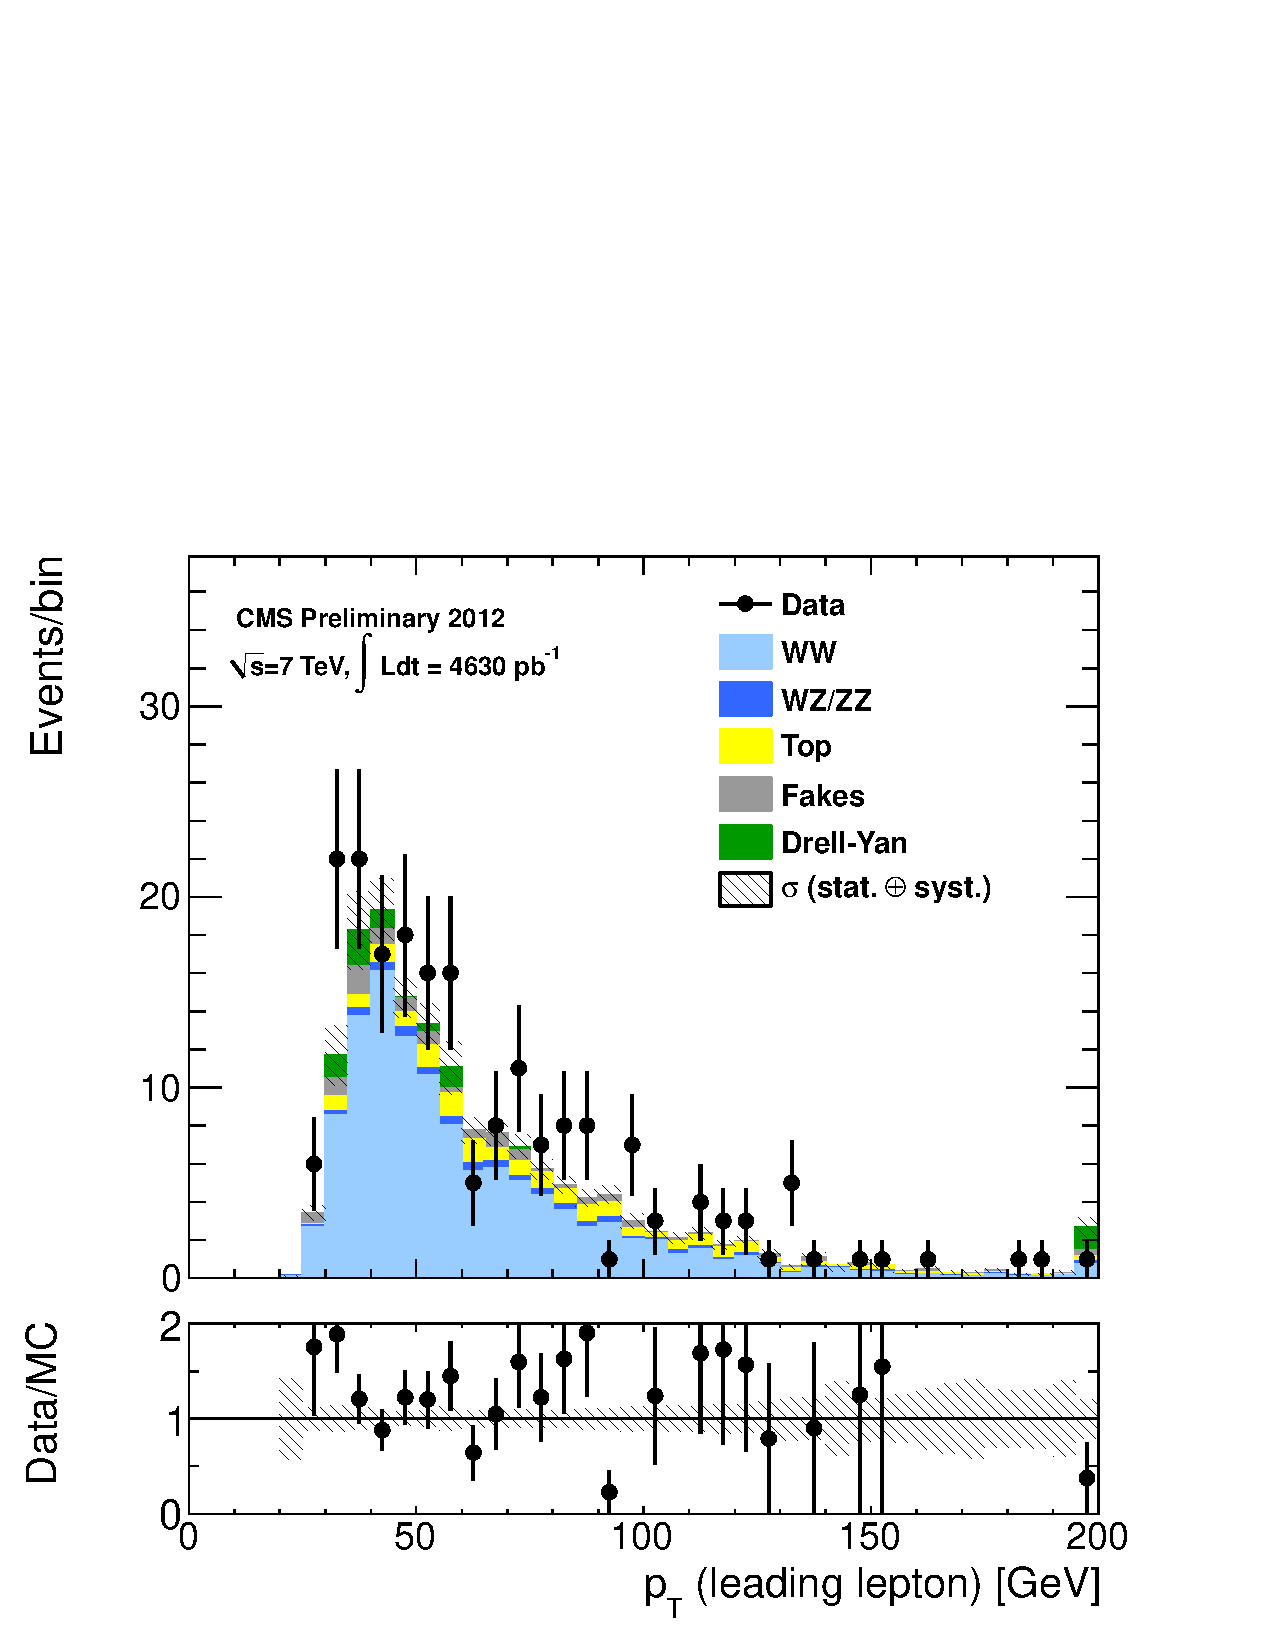
\includegraphics[width=.45\textwidth]{figures/pas_pt1_ee.pdf}}
\subfigure[Trailing lepton $p_{T}$]{\label{subfig:fig_eeplots_pt2}
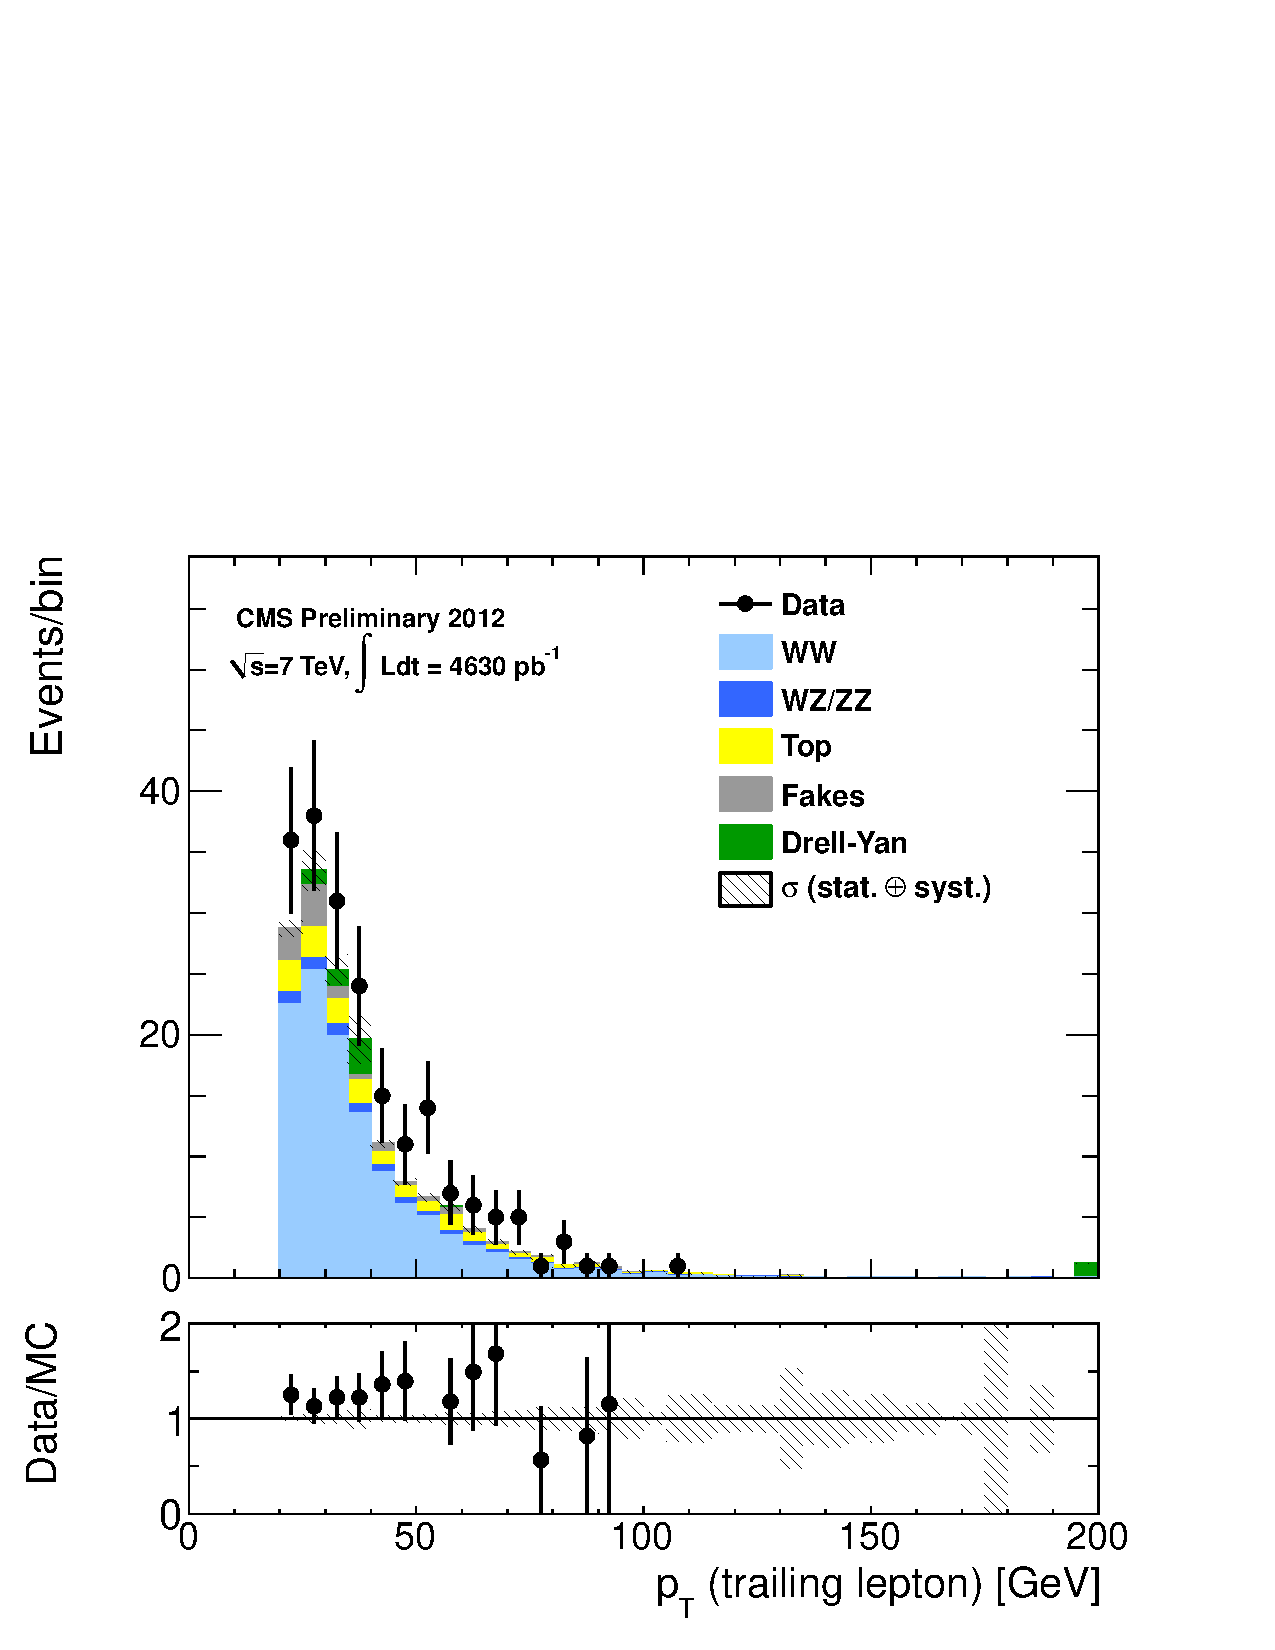
\includegraphics[width=.45\textwidth]{figures/pas_pt2_ee.pdf}}
\subfigure[Dilepton system $p_{T}$]{\label{subfig:fig_eeplots_ptll}
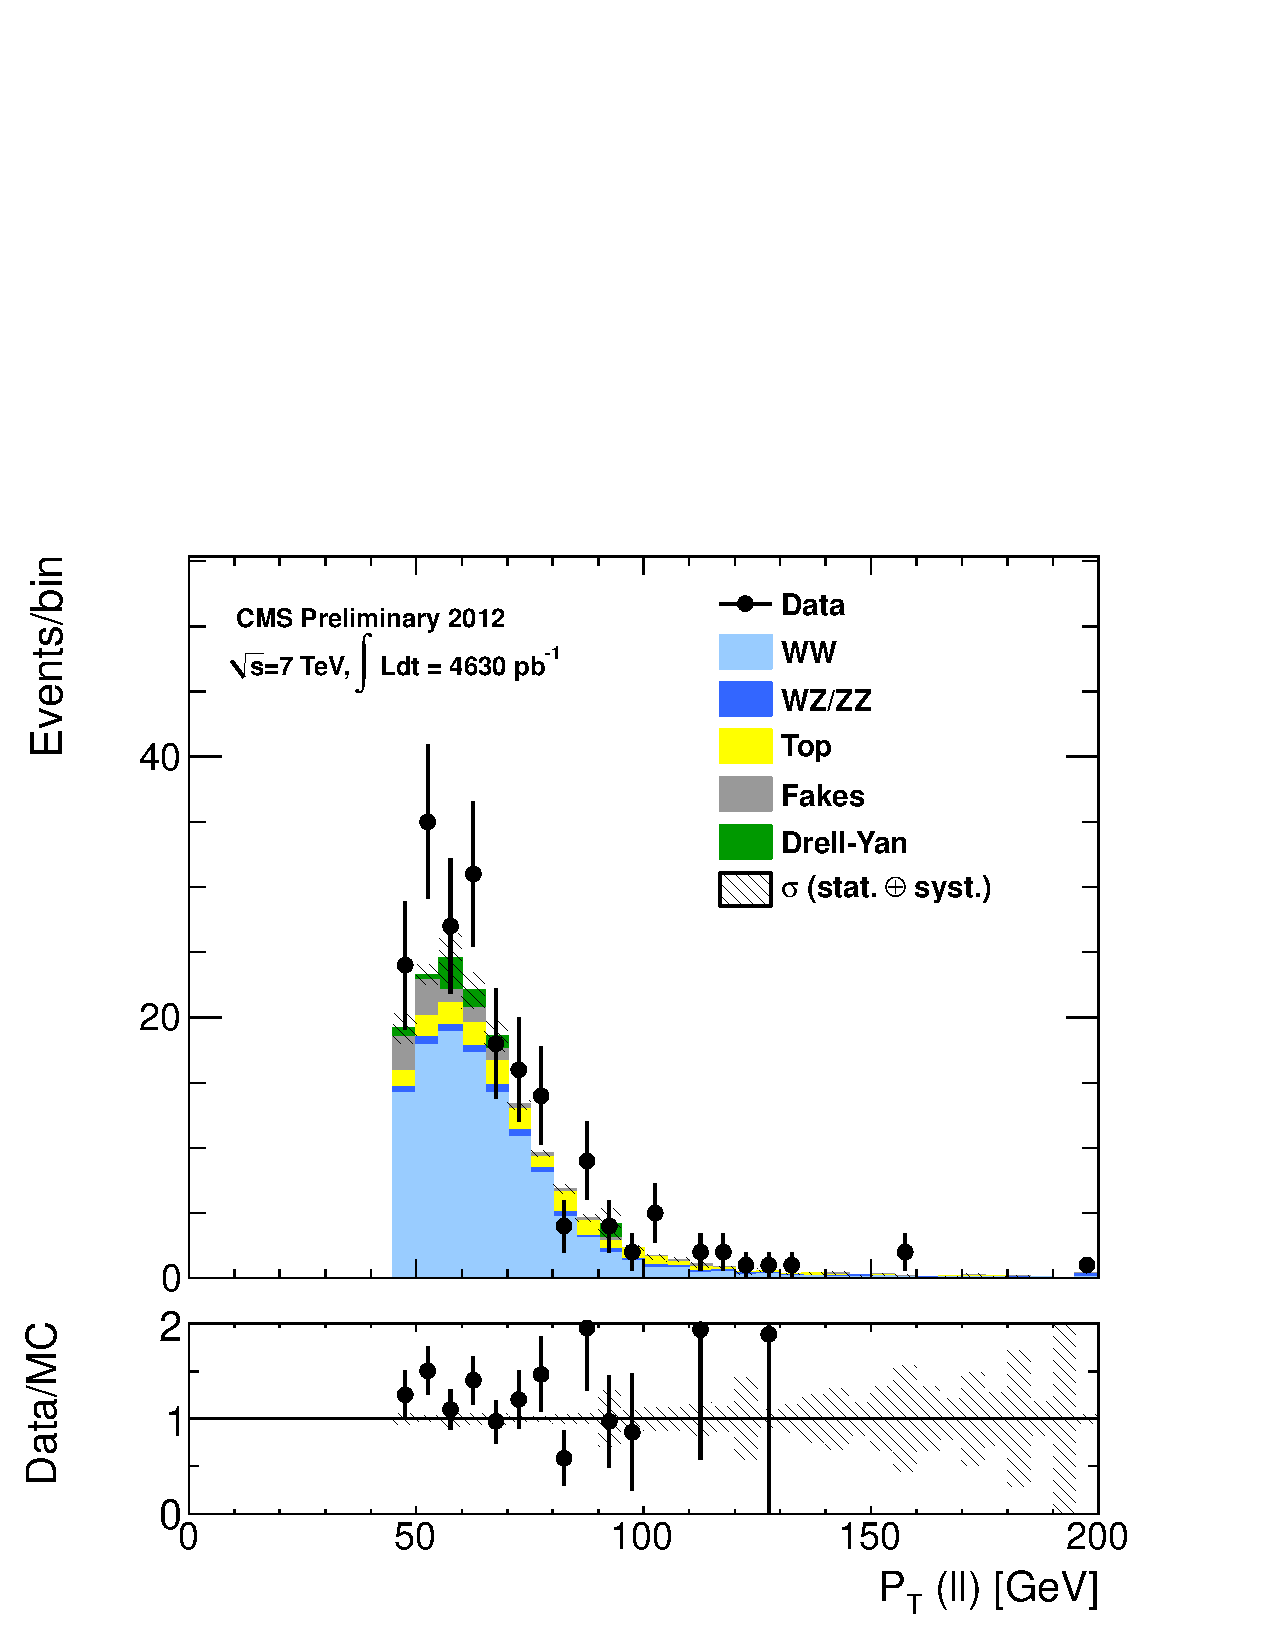
\includegraphics[width=.45\textwidth]{figures/pas_ptll_ee.pdf}}
\subfigure[Dilepton system invariant mass]{\label{subfig:fig_eeplots_M}
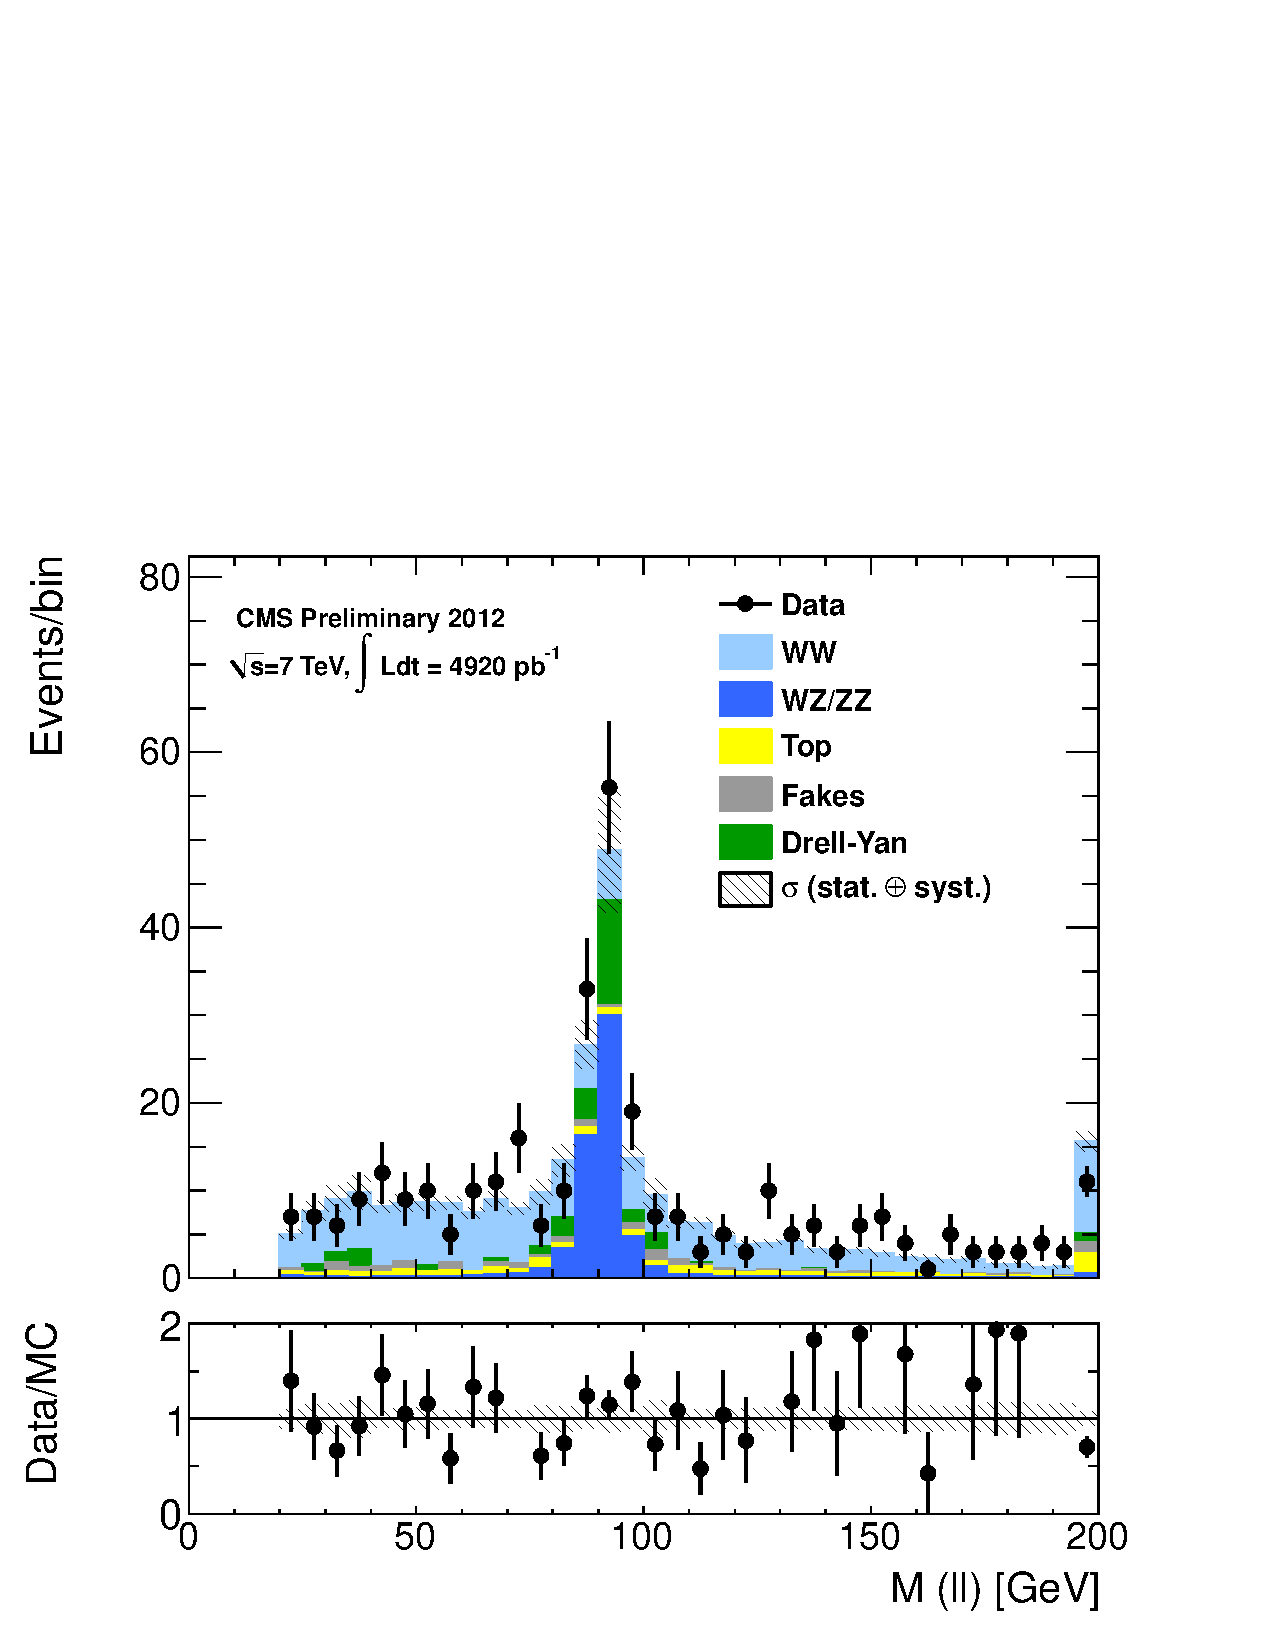
\includegraphics[width=.45\textwidth]{figures/pas_mll_ee.pdf}}
\caption{Kinematic distributions for expected and observed events in the $ee$ final state.
The dilepton system invariant mass distribution has the $Z$ mass veto relaxed.
The uncertainty on the expected events includes both statistical and systematic components.}
\label{fig:eeplots}
\end{center}
\end{figure}
%%%%%%%%

